\documentclass[a4paper]{article}
\usepackage[spanish]{babel}
\usepackage[utf8]{inputenc}
\usepackage{fancyhdr}
\usepackage{charter} % tipografia
%\usepackage{graphicx}
\usepackage[pdftex]{graphicx}
\usepackage{bm} % bold font in math mode
\usepackage{sidecap}
\usepackage{caption}
\usepackage{subcaption}
\usepackage{booktabs}
\usepackage{makeidx}
\usepackage{float}
\usepackage{amsmath, amsthm, amssymb}
\newtheorem{theorem}{Teorema}
\newtheorem{customthm}{Teorema}
\newtheorem{corollary}{Corolario}[theorem]
\newtheorem{proposition}[theorem]{Proposición}
\newtheorem{innercustomlemma}{Lemma}
\newenvironment{customlemma}[1]
  {\renewcommand\theinnercustomlemma{#1}\innercustomlemma}
  {\endinnercustomlemma}
\usepackage{amsfonts}
\usepackage{sectsty}
\usepackage{wrapfig}
\usepackage{listings}
\usepackage{hyperref} % links
\usepackage{algorithm} %http://www.ctan.org/pkg/algorithms
\usepackage{algorithmic}
\usepackage[usenames,dvipsnames]{xcolor}
\usepackage{pgfplots}
\usepackage{tabularx} % tablas copadas
% \usepackage{pgfplotstable}
% custom
\usepackage{color} % para snipets de codigo coloreados
\usepackage{fancybox} % para el sbox de los snipets de codigo
\definecolor{litegrey}{gray}{0.94}
% \newenvironment{sidebar}{%
% \begin{Sbox}\begin{minipage}{.85\textwidth}}%
% {\end{minipage}\end{Sbox}%
% \begin{center}\setlength{\fboxsep}{6pt}%
% \shadowbox{\TheSbox}\end{center}}
% \newenvironment{warning}{%
% \begin{Sbox}\begin{minipage}{.85\textwidth}\sffamily\lite\small\RaggedRight}%
% {\end{minipage}\end{Sbox}%
% \begin{center}\setlength{\fboxsep}{6pt}%
% \colorbox{litegrey}{\TheSbox}\end{center}}

%\newenvironment{codesnippet}{%
%\begin{Sbox}\begin{minipage}{\linewidth-2\fboxsep-2\fboxrule-4pt}\sffamily\small}%
%{\end{minipage}\end{Sbox}%
%\begin{center}%
%\colorbox{litegrey}{\TheSbox}\end{center}}

% \newenvironment{codesnippet}{\VerbatimEnvironment%
%   \noindent
%   %{\columnwidth-\leftmargin-\rightmargin-2\fboxsep-2\fboxrule-4pt}
%   \begin{Sbox}
%   \begin{minipage}{\linewidth-2\fboxsep-2\fboxrule-4pt}
%   \begin{Verbatim}
% }{%
%   \end{Verbatim}
%   \end{minipage}
%   \end{Sbox}%
%   \colorbox{litegrey}{\TheSbox}
% }

\newenvironment{codesnippet}{%
  \noindent
  %      {\columnwidth-\leftmargin-\rightmargin-2\fboxsep-2\fboxrule-4pt}
  \begin{Sbox}
  \begin{minipage}{\linewidth}
  \begin{lstlisting}
}{
  \end{lstlisting}
  \end{minipage}
  \end{Sbox}%
  \colorbox{litegrey}{\TheSbox}
}

\usepackage{fancyhdr}
\pagestyle{fancy}
%\renewcommand{\chaptermark}[1]{\markboth{#1}{}}
\renewcommand{\sectionmark}[1]{\markright{\thesection\ - #1}}
\fancyhf{}
\fancyhead[LO]{Sección \rightmark} % \thesection\
\fancyfoot[LO]{\small{Iv\'an Arcuschin, Mart\'in Jedwabny, Jos\'e Massigoge, Iv\'an Pondal}}
\fancyfoot[RO]{\thepage}
\renewcommand{\headrulewidth}{0.5pt}
\renewcommand{\footrulewidth}{0.5pt}
\setlength{\hoffset}{-0.8in}
\setlength{\textwidth}{16cm}
%\setlength{\hoffset}{-1.1cm}
%\setlength{\textwidth}{16cm}
\setlength{\headsep}{0.5cm}
\setlength{\textheight}{25cm}
\setlength{\voffset}{-0.7in}
\setlength{\headwidth}{\textwidth}
\setlength{\headheight}{13.1pt}
\renewcommand{\baselinestretch}{1.1} % line spacing

% -------------------- COMANDOS ESPECIALES ------------------------------

\newcommand{\calcular}[2]{\pgfmathtruncatemacro{#1}{#2}}

\pgfplotsset{
  filter params/.style n args={4}{
      x filter/.code={
          \edef\tempa{\thisrow{#1}}
          \edef\tempb{#2}
          \edef\tempc{\thisrow{#3}}
          \edef\tempd{#4}
          \ifx\tempa\tempb
            \ifx\tempc\tempd
            \else
              \def\pgfmathresult{inf}
            \fi
          \else
            \def\pgfmathresult{inf}
          \fi
      }
  }
}

\newcommand{\graficarDatos}[6]{
  \begin{tikzpicture}
  \begin{axis}[
      title={#1},
      xlabel={#2},
      ylabel={#3},
      scaled x ticks=false,
      scaled y ticks=false,
      scale=0.5
  ]
  \addplot[only marks, color=black] table[x=#4,y=#5]{#6};
  \end{axis}
  \end{tikzpicture}
}

\newcommand{\graficarDatosPlus}[7]{
  \begin{tikzpicture}
  \begin{axis}[
      title={#1},
      xlabel={#2},
      ylabel={#3},
      scaled x ticks=false,
      scaled y ticks=false,
      width=0.6\textwidth,
      #7
  ]
  \addplot[only marks, color=black] table[x=#4,y=#5]{#6};
  \end{axis}
  \end{tikzpicture}
}

\makeatletter
\pgfplotsset{
    groupplot xlabel/.initial={},
    every groupplot x label/.style={
        at={($({group c1r\pgfplots@group@rows.west}|-{group c1r\pgfplots@group@rows.outer south})!0.5!({group c\pgfplots@group@columns r\pgfplots@group@rows.east}|-{group c\pgfplots@group@columns r\pgfplots@group@rows.outer south})$)},
        anchor=north,
    },
    groupplot ylabel/.initial={},
    every groupplot y label/.style={
            rotate=90,
        at={($({group c1r1.north}-|{group c1r1.outer
west})!0.5!({group c1r\pgfplots@group@rows.south}-|{group c1r\pgfplots@group@rows.outer west})$)},
        anchor=south
    },
    execute at end groupplot/.code={%
      \node [/pgfplots/every groupplot x label]
{\pgfkeysvalueof{/pgfplots/groupplot xlabel}};
      \node [/pgfplots/every groupplot y label]
{\pgfkeysvalueof{/pgfplots/groupplot ylabel}};
    },
    group/only outer labels/.style =
{
group/every plot/.code = {%
    \ifnum\pgfplots@group@current@row=\pgfplots@group@rows\else%
        \pgfkeys{xticklabels = {}, xlabel = {}}\fi%
    \ifnum\pgfplots@group@current@column=1\else%
        \pgfkeys{yticklabels = {}, ylabel = {}}\fi%
}
}
}

\def\endpgfplots@environment@groupplot{%
    \endpgfplots@environment@opt%
    \pgfkeys{/pgfplots/execute at end groupplot}%
    \endgroup%
}
\makeatother

\newcommand{\barGraphExp}[2]{
    \begin{tikzpicture}
    \begin{axis}[
        xlabel={Implementación},
    	ylabel={Tiempo de ejecución (clocks)},
        legend style={at={(1.4,1.0)}},
        ybar,
        scaled ticks=false,
        width=0.5\textwidth,
        height=0.5\textwidth,
        tickpos=left,
        xtick=\empty,
        ytick align=inside,
        xtick align=inside,
    	enlargelimits=0.05,
        bar width=16,
    ]
    % How to process each item:
    \renewcommand*{\do}[1]{\addplot+[color=black] table[x=n, y=##1]{datos/datos_blur.dat};}
    % Process list:
    \docsvlist{#2}
    \legend{#2}
    \end{axis}
    \end{tikzpicture}
}

\newcommand{\graficarDatosExp}[6]{
  \begin{tikzpicture}
  \begin{axis}[
      title={#1},
      xlabel={#2},
      ylabel={#3},
      scaled x ticks=false,
      scaled y ticks=false,
      enlargelimits=0.05,
      width=0.5\textwidth,
      height=0.5\textwidth
  ]
  \addplot[color=black] table[x=#5,y=#6]{#4};
  % \renewcommand*{\do}[1]{\addplot table[x=#5,y=##1]{#4};}
  % %     % Process list:
  % \docsvlist{#6}
  % \legend{#6}
  \end{axis}
  \end{tikzpicture}
}

% ------------------------------------------------------------------------

% \setcounter{secnumdepth}{2}
\usepackage{underscore}
\usepackage{kbordermatrix}% Matrix column labels
\usepackage{caratula}
\usepackage{url}
\lstset{
    language=C++,
    basicstyle=\ttfamily,
    keywordstyle=\color{blue}\ttfamily,
    stringstyle=\color{red}\ttfamily,
    commentstyle=\color{ForestGreen}\ttfamily,
    morecomment=[l][\color{magenta}]{\#}
}
\DeclareUnicodeCharacter{2212}{-}

% *********************** %
\usepackage{tikz}
\usetikzlibrary{graphs}
\usetikzlibrary{calc}
\usetikzlibrary{arrows}
% Otros
\usepackage{arrayjobx}
\usepackage{enumitem}
\usepackage{multicol}
\usepackage{etoolbox}
\usepackage{listingsutf8}
\lstset{inputencoding=utf8/latin1}
\usepackage{fancyvrb}
%\newcommand{\noindex}{\hspace*{-0.8em}}%
\lstset{
	breaklines=true,
	literate={\ \ }{{\ }}1,
	tabsize=2}
\newcommand{\subscript}[2]{$#1 _ #2$}
% *********************** %

% ******************************************************** %
% TEMPLATE DE INFORME ORGA2 v0.1 %
% ******************************************************** %
% ******************************************************** %
% %
% ALGUNOS PAQUETES REQUERIDOS (EN UBUNTU): %
% ========================================
% %
% texlive-latex-base %
% texlive-latex-recommended %
% texlive-fonts-recommended %
% texlive-latex-extra %
% texlive-lang-spanish (en ubuntu 13.10) %
% ******************************************************** %
\begin{document}
\thispagestyle{empty}
\materia{Métodos Numéricos}
\submateria{Segundo Cuatrimestre de 2015}
\titulo{Trabajo Práctico II}
%\subtitulo{Grupo: }
\integrante{Iv\'an Arcuschin}{678/13}{iarcuschin@gmail.com}
\integrante{Mart\'in Jedwabny}{885/13}{martiniedva@gmail.com}
\integrante{Jos\'e Massigoge}{954/12}{jmmassigoge@gmail.com}
\integrante{Iv\'an Pondal}{078/14}{ivan.pondal@gmail.com}
\maketitle
% no footer on the first page
\thispagestyle{empty}
\newpage

\tableofcontents

\newpage
\section{Introducción}
 El objetivo principal de este Trabajo Práctico es estudiar, implementar y analizar
 algoritmos de Rankeo en dos escenarios distintos: tanto para páginas Web como para
 competencias deportivas.

Comenzaremos haciendo una breve introducción al algoritmo \textit{PageRank}, el cual
es muy conocido por ser utilizado por el buscador Google,
 para luego pasar a describir el Modelo que lo sostiene,
donde explicaremos como resuelve este algoritmo el problema de rankear
páginas web.

Luego, veremos una posible optimización de \textit{PageRank} al modelar
el problema de una manera equivalente utilizando matrices esparsas. Para esto,
presentaremos y analizaremos 3 estructuras de datos distintas que nos permitirán mejorar la
complejidad espacial y temporal de dicho algoritmo. Además, demostraremos que el Algortimo 1 propuesto en Kamvar et al.
para trabajar con matrices esparsas es correcto.

A continuación, presentaremos el Modelo del algoritmo \textit{GeM} (Generalized Markov chains Method) basado en
\textit{PageRank}. \textit{GeM}, a diferencia de su padre, no se orienta a páginas web, sino a competencias
deportivas, por lo que mostraremos los aspectos en los cuales difieren.
En particular, mostraremos el problema de considerar deportes con empates al utilizar \textit{GeM} y dos formas
alternativas de modelar dicho escenario.

Una vez finalizada la parte del Modelo, pasaremos a describir la Implementación de los
diferentes algoritmos presentados. Dichas implementaciones fueron relalizadas algunas en
\texttt{C++} y otras en \texttt{MATLAB/Octave}.

Ya llegando al final, pasaremos a presentar la Experimentación realizada, a la vez
que iremos analizando y discutiendo los resultados obtenidos.

Los experimentos realizados para \textit{PageRank} fueron:
\begin{itemize}
    \item Convergencia del algoritmo.
    \item Tiempos de ejecución.
    \item Calidad de los resultados.
\end{itemize}

Y para \textit{GeM}:
\begin{itemize}
    \item Variación del parámetro $c$.
    \item Evolución del ranking por cada iteración.
\end{itemize}

Para finalizar, cerraremos el presente informe con una conclusión, en la cual
discutiremos acerca de los algoritmos vistos, así como de la experimentación realizada.
También, contaremos las dificultades encontradas al realizar el Trabajo Práctico,
las posibles continuaciones que se podrían realizar, y si los objetivos planteados
fueron alcanzados.


\newpage
\section{Modelo}
\subsection{Rankings de Páginas Web}

Hoy en día la cantidad de páginas web en todo el mundo asciende a una cantidad de
4.79 billones (sólo las indexadas). Es por esta razón que los buscadores
(Search Engines) cumplen un rol tan importante en el uso diario de internet desde
hace muchos años.

Dichos buscadores nos permiten realizar busquedas de páginas web mediante distintos
criterios, facilitando el acceso a la información.

Un posible criterio (bastante utilizado) es considerar que las páginas web populares
son las más buscadas. De esta forma, el buscador puede ofrecernos en orden descendiente
de popularidad los resultados obtenidos, esperando que encontremos más rápido lo
 que buscamos.

 Siguiendo esta intuición, se han elaborado diferentes algoritmos para ``rankear''
 las páginas web. A continuación presentaremos el famoso método PageRank, utilizado
 por Google en sus comienzos.

\subsubsection{PageRank}\label{PageRank}

El algoritmo de PageRank\footnote{Kurt Bryan and Tanya Leise. The linear algebra
behind google. SIAM Review, 48(3):569–581, 2006.} se define para un conjunto de
páginas Web $ = \{ 1,\dots, n \}$ de forma tal de asignar a cada una de ellas un
 puntaje que determine la importancia relativa de la página respecto de las demás.

Llamemos $x_j$ al puntaje asignado a la página $j\in\ Web$, que es lo que buscamos
calcular.

Ahora, un link saliente de la página $j$ a la página $i$ puede significar que $i$
 es una página importante. Pero bien podría ser que $j$ sea una página muy poco
 importante, por lo que deberíamos ponderar sus links salientes para decidir
 la importancia de las páginas a las que apunta.

Luego, vamos a considerar que la importancia de la página $i$ obtenida mediante el
link de $j$ es proporcional a la importancia de $j$ e inversamente proporcional
al grado de $j$. Entonces, si $L_k \in\ Web$ es el conjunto de páginas web que
apuntan a la página $k$:

\begin{equation} \label{eq:puntajes_page_rank}
    x_k = \sum\limits_{j \in\ L_k}{\frac{x_j}{n_j}},\quad k=1,\dots,n
\end{equation}

En este algoritmo, hallaramos los $x_k$ modelando el problema como una cadena de
 Markov, a la cual llamaremos Matriz de Transición, y que construiremos de la siguiente forma:

\begin{enumerate}
	\item Sea $G$ el grafo de la Web, dónde cada vértice es una página web y un
		eje de $v$ a $u$ significa que la página $v$ tiene link saliente hacia $u$.
	\item Luego, sea $W\in\{0,1\}^{n \times n}$ la \textit{matriz de conectividad} de $G$, tal
        que la celda $\{i,j\}$ tiene un 1 si hay un link saliente de la $j$-ésima página
        a la $i$-ésima página (los \textit{autolinks} son ignorados, o lo que es lo mismo,
        $\forall\ 1\leq i\leq n\ W_{i,i}$).
	\item Si definimos $n_j = \sum\limits_{i=1}^{n}{W_{i,j}}$ como el grado de $j$
        (la cantida de links salientes), entonces podemos definir la matriz
        $P\in\mathbb{R}^{n \times n}$, tal que la $P_{i,j} = 1/n_{j} * W_{i,j} $, y
        $P$ es estocástica por columnas.

        Además, notese que resolver el sistema dado por \ref{eq:puntajes_page_rank}
        es equivalente a encontrar un $x\in\mathbb{R}^n$ tal que $Px=x$.
        Es decir, encontrar el autovector asociado al autovalor 1 de $P$ tal que
        $x_i > 0$ y $\sum\limits_{i=1}^{n}{x_i} = 1$.
    \item Ahora, puede pasar que para algún $j$, $n_j = 0$ lo que indicaría que
        la página $j$ no tiene ningún link saliente. Para remediar
        estos casos, vamos a modificar $P$ utilizando la idea del  \textit{navegante
        aleatorio}, de forma tal que para un $j$ sin links salientes, la probabilidad
        de que el navegante salte a cualquier otra página $i$ es $1/n$.

        Entonces, $P_{1} = P + D$, dónde $D = vd^{t}$, $d\in\{0,1\}^{n}$ tal que
        $d_j = 1$ si $n_j = 0$, y $d_j = 0$ en caso contrario, y $v\in\mathbb{R}^n$
         tal que $v_j = 1/n$.
    \item Entonces, $P_{1}$ es estocástica por columnas, pero puede que no sea regular.
        Para que sí lo sea, extendemos el concepto anterior a todas las páginas
        (fenómeno de \textit{teletransportación}).

        Luego, $P_{2} = c*P_{1} + (1-c)*E$, donde $\forall\ 1\leq i,j\leq n,\ E_{i,j} = 1/n$,
        y $c\in(0,1)$. Llamamos a $c$ coeficiente de teletransportación.

        Lo que nos queda es un matriz $P_{2}$ estocástica por columnas y $\forall\ 1\leq i,j\leq n,\ (P_{2})_{i,j} > 0$.
\end{enumerate}

Una vez que tenemos la Matriz de Transición, generaremos el puntaje para cada página
 buscando el autovector $w$ del autovalor 1 de $P_{2}$, tal que $P_{2}w = w$ y
$w$ sea un vector de probabilidades (normalizado con norma 1).

Es decir, generar el ranking de páginas equivale a aplicar el método de la potencia
a la matriz $P_{2}$ y una vez hallado el $w$ mencionado, ordenar los puntajes de
mayor a menor:

\begin{equation} \label{eq:ranking_page_rank}
    ranking = \{ p_1, \dots, p_n \}, \text{donde } \forall\ i=1,\dots,n-1,\ w_{p_{i}} \geq w_{p_{i+1}}
\end{equation}

\subsubsection{PageRank con matriz Esparsa}

Partiendo del hecho de que, aproximadamente, cada pagina Web tiene 7 links salientes\footnote{Sepandar D. Kamvar, Taher H. Haveliwala, Christopher D. Manning, and Gene H. Golub.
Extrapolation methods for accelerating pagerank computations. In Proceedings of the 12th
international conference on World Wide Web, WWW ’03, pages 261–270, New York, NY,
USA, 2003. ACM.} surge la posibilidad de optimizar la estructura que representa el Grafo dirigido de la Web, debido a la baja densidad de la matriz de conectividad, $W$, asociada a dicho Grafo.
Esta optimizacion no es solo una posibilidad, sino una necesidad dado que la cantidad de Webs indexadas tiene un requerimiento prohibitivo en terminos de memoria si la representamos, ingenuamente, como un vector de vectores.
Nuestra hipotesis es que, utilizando una estructura de datos optimizada, no solo obtendremos mejoras en terminos de complejidad espacial, sino tambien en terminos de complejidad temporal.

A partir de este analisis, nos propusimo analizar tres estructuras de datos que representan matrices esparsas:
\begin{enumerate}
  \item \textit{Dictionary of Keys (dok)}
  \item \textit{Compressed Sparse Row (CSR)}
  \item \textit{Compressed Sparse Column (CSC)}
\end{enumerate}

Sea $A \in \mathbb{R}^{n \times n}$ una matriz esparsa, y sea $m$ es la cantidad de valores distintos de 0 de $A$.
\paragraph{1. Dictionary of Keys (dok):}
Esta estructura esta representada como un vector de diccionarios, en donde cada posicion, $i$, del vector puede considerarse como una fila, y la key del diccionario contenido dentro de esa posicion representa una columna, $j$, siendo el valor asociado a esa key, en el diccionario, el valor en la matriz contenido en esa fila y columna ($A_{ij}$). Solo aquellas $A_{ij}$ que tienen valores distintos de 0 tienen una key en los diccionarios.
\newline
\newline
Veamos un ejemplo. Sea $B \in \mathbb{R}^{4 \times 4}$ la siguiente matriz:
\[
  B = \left(\begin{array}{*5{c}}
    10 & 0 & 0 & -2\\
    3  & 9 & 0 & 0 \\
    0  & 7 & 8 & 0 \\
    3  & 0 & 4 & 5
  \end{array}\right)
\]
El dictionary of keys que representa a $B$ es:
\def\leftbracket{[}
\def\rightbracket{]}

\begin{center}
\tikzset{my arrow/.style={
  blue!60!black,
  -latex
  }
}

\begin{tikzpicture}
\matrix[matrix of math nodes, row sep=4mm] (M) {
\leftbracket & 1 & 2 & 3 & 4 & \rightbracket \\
\leftbracket & a_1 & a_2 & a_4 & a_3 & \rightbracket \\
\leftbracket & a_1 & a_4 & a_2 & a_3 & \rightbracket \\
};

\draw[my arrow] (M-3-3) to (M-2-4);
\draw[my arrow] (M-1-4) to (M-2-4);
\end{tikzpicture}

\end{center}

\begin{tikzpicture}

\tikzset{square matrix/.style={
    matrix of nodes,
    column sep=-\pgflinewidth, row sep=-\pgflinewidth,
    nodes={draw,
      minimum height=#1,
      anchor=center,
      text width=#1,
      align=center,
      inner sep=0pt
    },
  },
  square matrix/.default=1.2cm
}

\matrix[square matrix]
{
\text{[1;10] [5;-2]} & \text{[1;3] [2;9]} & 11 & 8 & 5 \\
};
\end{tikzpicture}
\newline
Esta claro que intercambiando columnas por filas, como posiciones del vector contenedor, y filas por columnas como keys, representamos la misma matriz.
\newline
\newline
Las ventajas de usar esta estructura de datos son las siguientes:
\begin{enumerate}
  \item Facilidad para crearse de forma dinamicamente, es decir, si a priori no conocemos la forma de la matriz a representar.
  \item La operacion matriz esparsa por vector es sencilla.
\end{enumerate}
Por otro lado, sus desventajas son:
\begin{enumerate}
  \item Los accesos a los valores no tienen complejidad temporal constante.
  \item Las operaciones entre matrices esparsas, sea la suma o la multiplicacion, son engorrosas.
\end{enumerate}

\paragraph{2. Compressed Sparse Row (CSR):}

Esta estructura utiliza tres vectores, dos de tamano $m$, llamemosles \textit{val} y \textit{col_ind} respectivamente, y uno de tamano $n+1$, llamemosle \textit{row_ptr}.
\begin{itemize}
    \item En \textit{val} guardamos los valores de $A$ distintos de 0, recorriendo $A$ por filas, es decir fijando las filas y avanzado por las columnas.
    \item En la posicion $k$ de \textit{col_ind} guardamos el indice $j$ del valor $A_{ij}$ contenido en la posicion $k$ del vector \textit{val}.
    \item Por ultimo en \textit{row_ptr} guardamos indices del vector \textit{val} en los cuales se encuentran el primera valor de cada fila, de tal
     forma que para la fila $i$, el valor $k$ contenido en \textit{row_ptr[i]}, nos dice que \textit{val[k]} corresponde al primer valor de la fila
      $i$ y el valor $k'$ contenido en \textit{row_ptr[i+1]}, nos dice que \textit{val[k'-1]} corresponde al ultimo valor de la fila $i$.
      Vale la pena aclarar que si $k = k'$ entonces la fila no tiene valores distintos de 0.
\end{itemize}

Utilizemos $B$ como la matriz del punto anterior:
\[
  B = \left(\begin{array}{*5{c}}
    10 & 0 & 0 & -2\\
    3  & 9 & 0 & 0 \\
    0  & 7 & 8 & 0 \\
    3  & 0 & 4 & 5
  \end{array}\right)
\]

La misma seria representado de la siguiente manera:
\begin{itemize}
  \item \textit{val:}
\end{itemize}
\begin{center}
\begin{tikzpicture}
\tikzset{square matrix/.style={
    matrix of nodes,
    column sep=-\pgflinewidth, row sep=-\pgflinewidth,
    nodes={draw,
      minimum height=#1,
      anchor=center,
      text width=#1,
      align=center,
      inner sep=0pt
    },
  },
  square matrix/.default=0.8cm
}

\matrix[square matrix]
{
10 & -2 & 3 & 9 & 7 & 8 & 3 & 4 & 5 \\
};
\end{tikzpicture}
\end{center}

\begin{center}
\begin{itemize}
  \item \textit{col_ind:}
\end{itemize}
\begin{tikzpicture}

\tikzset{square matrix/.style={
    matrix of nodes,
    column sep=-\pgflinewidth, row sep=-\pgflinewidth,
    nodes={draw,
      minimum height=#1,
      anchor=center,
      text width=#1,
      align=center,
      inner sep=0pt
    },
  },
  square matrix/.default=0.8cm
}

\matrix[square matrix]
{
1 & 5 & 1 & 2 & 2 & 3 & 1 & 3 & 5 \\
};
\end{tikzpicture}
\end{center}

\begin{center}
\begin{itemize}
  \item \textit{row_ptr:}
\end{itemize}

\begin{tikzpicture}

\tikzset{square matrix/.style={
    matrix of nodes,
    column sep=-\pgflinewidth, row sep=-\pgflinewidth,
    nodes={draw,
      minimum height=#1,
      anchor=center,
      text width=#1,
      align=center,
      inner sep=0pt
    },
  },
  square matrix/.default=0.8cm
}

\matrix[square matrix]
{
1 & 3 & 5 & 7 & 10 \\
};
\end{tikzpicture}
\end{center}

Las ventajas de usar esta estructura de datos son las siguientes:
\begin{enumerate}
  \item Eficiente a la hora de realizar operaciones aritmeticas entre matrices esparsas (suma, multiplicacion).
  \item La operacion matriz esparsa por vector es sencilla.
\end{enumerate}
Por otro lado, sus desventajas son:
\begin{enumerate}
  \item Dificultad a la hora de crearse de forma dinamica, ya que debemos recalcular/redimensionar los tamanos de los vectores.
  \item Cambios en la esparcidad son costosos, misma razon que el punto anterior.
\end{enumerate}

\paragraph{3. Compressed Sparse Column (CSC):}

Muy parecidad a la \textit{Compressed Sparse Row (CSR)}.
 Tambien utiliza tres vectores, dos de tamano $m$, llamemosles \textit{val} y \textit{row_ind} respectivamente, y uno de tamano $n+1$, llamemosle \textit{col_ptr}.

 \begin{itemize}
     \item En \textit{val} guardamos los valores de $A$ distintos de 0, recorriendo $A$ por columnas, es decir fijando las columnas y avanzado por las filas.
     \item En la posicion $k$ de \textit{row_ind} guardamos el indice $i$ del valor $A_{ij}$ contenido en la posicion $k$ del vector \textit{val}.
     \item Por ultimo en \textit{col_ptr} guardamos indices del vector \textit{val} en los cuales se encuentran el primera valor de cada columna, de tal forma que para la columna $j$, el valor $k$ contenido en \textit{col_ptr[j]}, nos dice que \textit{val[k]} corresponde al primer valor de la fila $j$ y el valor $k'$ contenido en \textit{col_ptr[j+1]}, nos dice que \textit{val[k'-1]} corresponde al ultimo valor de la col $j$. Vale la pena aclarar que si $k = k'$ entonces la columna no tiene valores distintos de 0.
 \end{itemize}

Nuevamente utilizemos $B$ como ejemplo:
\[
  B = \left(\begin{array}{*5{c}}
    10 & 0 & 0 & -2\\
    3  & 9 & 0 & 0 \\
    0  & 7 & 8 & 0 \\
    3  & 0 & 4 & 5
  \end{array}\right)
\]

La misma seria representado de la siguiente manera:
\begin{itemize}
  \item \textit{val:}
\end{itemize}

\begin{center}
\begin{tikzpicture}
\tikzset{square matrix/.style={
    matrix of nodes,
    column sep=-\pgflinewidth, row sep=-\pgflinewidth,
    nodes={draw,
      minimum height=#1,
      anchor=center,
      text width=#1,
      align=center,
      inner sep=0pt
    },
  },
  square matrix/.default=0.8cm
}

\matrix[square matrix]
{
10 & 3 & 3 & 9 & 7 & 8 & 4 & -2 & 5 \\
};
\end{tikzpicture}
\end{center}

\begin{center}
\begin{itemize}
  \item \textit{row_ind:}
\end{itemize}
\begin{tikzpicture}

\tikzset{square matrix/.style={
    matrix of nodes,
    column sep=-\pgflinewidth, row sep=-\pgflinewidth,
    nodes={draw,
      minimum height=#1,
      anchor=center,
      text width=#1,
      align=center,
      inner sep=0pt
    },
  },
  square matrix/.default=0.8cm
}

\matrix[square matrix]
{
1 & 2 & 4 & 2 & 3 & 3 & 4 & 1 & 4 \\
};
\end{tikzpicture}
\end{center}

\begin{center}
\begin{itemize}
  \item \textit{col_ptr:}
\end{itemize}

\begin{tikzpicture}

\tikzset{square matrix/.style={
    matrix of nodes,
    column sep=-\pgflinewidth, row sep=-\pgflinewidth,
    nodes={draw,
      minimum height=#1,
      anchor=center,
      text width=#1,
      align=center,
      inner sep=0pt
    },
  },
  square matrix/.default=0.8cm
}

\matrix[square matrix]
{
1 & 4 & 6 & 8 & 10 \\
};
\end{tikzpicture}
\end{center}

Las ventajas de usar esta estructura de datos son las siguientes:
\begin{enumerate}
  \item Eficiente a la hora de realizar operaciones aritmeticas entre matrices esparsas (suma, multiplicacion).
  \item La operacion matriz esparsa por vector es sencilla.
\end{enumerate}
Por otro lado, sus desventajas son:
\begin{enumerate}
  \item Dificultad a la hora de crearse de forma dinamica, ya que debemos recalcular/redimensionar los tamanos de los vectores.
  \item Cambios en la esparcidad son costosos, misma razon que el punto anterior.
\end{enumerate}

\paragraph{Contexto de Uso}

Antes de definir que estructura de datos vamos a utilizar para representar matrices esparsas, debemos definir el contexto de uso de la misma.
Sabemos que el algoritmo de PageRank utiliza el metodo de la Potencia, usando la matriz $P_2$ definida previamente. Sin embargo la $P_2$ no es esparsa, inclusive todos sus valores son distintos de 0, por lo cual utilizar la implementacion del Page Rank descripta en la Seccion \ref{PageRank} no es posible .

Para poder hacer frente a esta dificultad, utilizamos el algoritmo propuesto por Kamvar et al.[Algoritmo 1]\footnote{Sepandar D. Kamvar, Taher H. Haveliwala, Christopher D. Manning, and Gene H. Golub.
Extrapolation methods for accelerating pagerank computations. In Proceedings of the 12th
international conference on World Wide Web, WWW ’03, pages 261–270, New York, NY,
USA, 2003. ACM.} para calcular $x^{(k+1)} = P_2x^{k}$, cuyos pasos son los siguientes:
\begin{enumerate}
    \item $y = cPx$
    \item $w = ||x||_1 - ||y||_1$
    \item $y = y + wv$
\end{enumerate}

donde $c$, $P$ y $v$ corresponden al escalar, la matriz y el vector descriptos en la Seccion \ref{PageRank}.

Tenemos que ver que el algortimo descripto calcula efectivamente $x^{(k+1)} = P_2x^{k}$:
\begin{proposition}
    El Algoritmo 1 calcula $x^{(k+1)} = P_2x^{(k)}$
\end{proposition}
\begin{proof}
Por definicion sabemos que
  \begin{equation*}
            \begin{aligned}
              x^{(k+1)} &= P_2x^{(k)} \\
               &= (cP_1 +(1-c)E)x^{(k)} \\
               &= (cP + cD +(1-c)E)x^{(k)} \\
               &= (cP + cD +(1-c)E)x^{(k)} \\
               &= (cP + cvd^{t} +(1-c)v1^{t})x^{(k)} \\
               &= cPx^{(k)} + cvd^{t}x^{(k)} +(1-c)v1^{t}x^{(k)} \\
            \end{aligned}
\end{equation*}
Por otro lado, el Algoritmo 1 nos dice que:
\begin{equation*}
          \begin{aligned}
            x^{(k+1)} &= cPx^{(k)} + (||x^{(k)}||_1 - ||cPx^{(k)}||_1)v  \\
          \end{aligned}
\end{equation*}
Luego basta ver que:
\begin{equation*}
          \begin{aligned}
            cPx^{(k)} + (||x^{(k)}||_1 + ||cPx^{(k)}||_1)v &= cPx^{(k)} + cvd^{t}x^{(k)} +(1-c)v1^{t}x^{(k)}  \\
            (||x^{(k)}||_1 - ||cPx^{(k)}||_1)v &= cvd^{t}x^{(k)} +(1-c)v1^{t}x^{(k)}  \\
            ||x^{(k)}||_1v - ||cPx^{(k)}||_1v &= cvd^{t}x^{(k)} +v1^{t}x^{(k)} - cv1^{t}x^{(k)}  \\
          \end{aligned}
\end{equation*}
Sabemos que $\forall\ 1\leq i\leq n\ x^{(k)}_{i} \geq 0$, ya que $x$ es un vector de probabilidades. Entonces $||x^{(k)}||_1$ = $\sum\limits_{i=1}^{n}{x^{(k)}_{i}}$. Tambien sabemos que $1^{t}x^{(k)} = \sum\limits_{i=1}^{n}{1x^{(k)}_{i}}$, por lo tanto
$||x^{(k)}||_1 = 1^{t}x^{(k)}$.
\newline
Por otro lado sabemos que $0\leq c\leq 1$, lo que implica que $|c| = c$.
\newline
Teniendo en cuenta esta informacion, la igualdad nos queda de la siguiente forma:
\begin{equation*}
          \begin{aligned}
            v1^{t}x^{(k)} - c||Px^{(k)}||_1v &= cvd^{t}x^{(k)} + v1^{t}x^{(k)} - cv1^{t}x^{(k)}  \\
            - c||Px^{(k)}||_1v &= cvd^{t}x^{(k)} - cv1^{t}x^{(k)}  \\
          \end{aligned}
\end{equation*}
Tomando como factor comun $v$ y $c$:
\begin{equation*}
          \begin{aligned}
            - c||Px^{(k)}||_1v &= cv(d^{t}x^{(k)} - 1^{t}x^{(k)})  \\
            - ||Px^{(k)}||_1 &= d^{t}x^{(k)} - 1^{t}x^{(k)}  \\
            - ||Px^{(k)}||_1 &= (d^{t} - 1^{t})x^{(k)}  \\
          \end{aligned}
\end{equation*}

Sabemos, por definicion de $d$, que $d^{t}$ solo tiene $1$ y $0$ como valores, por lo tanto al realizar $(d^{t} - 1^{t})$ obtendremos un vector fila,
llamemosle $z$, cuyos valores seran $0$ o $-1$. Lo que implica que $z_j = 0$ cuando $d^{t}_j = 1$, situacion que se da cuando, para ese
$j$, $\sum_{i=1}^{n}{P_{ij}} = 0$. Caso contrario $z_j = -1$ cuando $d^{t}_j = 0$, situacion que se da cuando, para ese $j$,
 $\sum_{i=1}^{n}{P_{ij}} = 1$. Por lo tanto al mutiplicar $zx^{(k)}$ obtendremos un escalar que sera la suma de los opuestos de
 los $x^{(k)}_j$ que cumplan que, para ese $j$, $\sum_{i=1}^{n}{P_{ij}} = 1$, ya que los otros seran mutiplicados por $0$.

Por otro lado, partiendo del hecho de que $P$ es estocastica por columnas, sabemos que al realizar $Px^{(k)}$, aquellas columnas, $j$, que
cumplan que $\sum_{i=1}^{n}{P_{ij}} = 0$, forzaran a que los $x^{(k)}_j$ no sean parte de ninguna componente del vector resultante,
ya que en todas las multiplicaciones de filas de $P$ por el vector $x^{(k)}$, estos $x^{(k)}_j$ seran multiplicados por $0$. Caso contrario
cuando las columnas, $j$, cumplan que $\sum_{i=1}^{n}{P_{ij}} = 1$, estas forzaran a que la suma de todos los $x^{(k)}_j$ presentes
en las distintas componentes del vector resultante sea igual a $x^{(k)}_j$. Precisamente al aplicar $||.||_1$ al vector $Px^{(k)}$, el
resultado sera un escalar que sera la suma de todas los $x^{(k)}_j$ que cumplan la condicion antes descripta. Por ultimo si al resultado
de aplicar $||.||_1$ lo multiplicamos por $-1$ obtenemos un escalar que sera la suma de los opuestos de los $x^{(k)}_j$ que cumplan que,
para ese $j$, $\sum_{i=1}^{n}{P_{ij}} = 1$.

Por todo lo expuesto anteriormente, podemos concluir que $- ||Px^{(k)}||_1 = (d^{t} - 1^{t})x^{(k)}$, lo que implica que El Algoritmo 1
calcula $x^{(k+1)} = P_2x^{(k)}$.
\end{proof}

Luego, sabemos que la unica operacion que vamos a realizar con la matriz esparsa es multiplicarla por un vector. Tambien sabemos que la
construccion de la matriz es de forma dinamica, ya que vamos leyendo los links salientes de cada pagina de forma secuencial.

A partir de esta informacion concluimos que la estructura de datos que mas se adecua a nuestras necesidades es el \textit{Dictionary
of Keys (dok)}, en donde las posiciones del vector representan las filas y las keys de los diccionarios las columnas.

Esta eleccion se debe al hecho de que podemos actualizar la matriz de forma sencilla a medida de que vamos leyendo los datos de entrada, y a su vez
 la multiplicacion por un vector se realiza de forma sencilla, vease Seccion Implementacion Esparsa (CAMBIAR CON LA REF).





\subsection{Rankings en competencias deportivas}

Elegir un sistema de puntos que sea justo para todos los participantes en un
deporte no es una tarea sencilla. Existen muchos factores que afectan el
resultado de una competencia como lo pueden ser el orden en el que deben
competir entre si los equipos, generando desbalances respecto las capacidades de
cada uno. Es por esto que a continuación presentaremos el modelo GeM
\footnote{Angela Y. Govan, Carl D. Meyer, and Rusell Albright. Generalizing
google’s pagerank to rank national football league teams. In Proceedings of SAS
Global Forum 2008, 2008.} que busca modelar los resultados de forma tal que estos
factores impacten lo menos posible en el posicionamiento final de la tabla de
puntajes.

Con el fin de experimentar con distintos modelos, a lo largo del informe
trabajaremos sobre los resultados del Torneo de Primera División
2015\footnote{Campeonato de Primera División 2015, \textit{Julio H. Grondona} \\
\url{http://www.afa.org.ar/html/9/estadisticas-de-primera-division}}, donde
utilizaremos el sistema de ranking estándar de la AFA como punto de comparación.

\subsubsection{Generalized Markov chains Method (GeM)}
\label{sec:gem_model}

\subsubsection*{Definición del método}

El método GeM es el resultado de tomar el algoritmo PageRank y mediante pequeñas
modificaciones utilizar su potencial para establecer un ranking de equipos.
Análogo a PageRank, los equipos pasan a formar parte de un grafo dirigido
con pesos, donde cada nodo representa un equipo y los pesos de cada arista
reflejan el resultado de los partidos jugados entre los vértices conectados.

~

Formalmente, el modelado se realiza de la siguiente manera:
\begin{enumerate}
	\item Representamos el torneo como un grafo con pesos dirigidos de $n$
	nodos, donde $n$ es igual a la cantidad de equipos que participan. Cada
	equipo tiene su respectivo nodo y las aristas contienen como peso la
	diferencia positiva entre los nodos conectados.

	\item Definimos la matriz de adyacencia $A \in \mathbb{R}^{n \times n}$.
		\begin{equation*}
			A_{ij} =
				\begin{cases}
					w_{ij} & \text{si el equipo $i$ perdió contra $j$}\\
					0 & \text{caso contrario}
				\end{cases}
		\end{equation*}
		Donde $w_{ij}$ es la suma total de diferencia positiva de puntaje sobre todos
		los partidos en los que $i$ perdió contra $j$.

	\item Definimos la matriz $H \in \mathbb{R}^{n \times n}$.
		\begin{equation*}
			H_{ij} =
				\begin{cases}
					A_{ij}/\sum_{k = 1}^{n}A_{ik} & \text{si hay un link de $i$ a $j$}\\
					0 & \text{caso contrario}
				\end{cases}
		\end{equation*}

	\item Definimos la matriz GeM, $G \in \mathbb{R}^{n \times n}$ con $u, v, a, e \in \mathbb{R}^n$ y $c \in \mathbb{R}$.
		\begin{gather*}
			G = c(H + au^{t}) + (1 - c)ev^{t} \\
			\sum_{k = 1}^{n}v_{k} = 1 \qquad \sum_{k = 1}^{n}u_{k} = 1 \qquad \forall_{i = 1..n} e_{i} = 1 \\
			0 \leq c \leq 1 \qquad
			a_{i} =
			\begin{cases}
				1 & \text{si la fila $i$ de $H$ es un vector nulo} \\
				0 & \text{caso contrario}
			\end{cases}
		\end{gather*}

	\item Por último tenemos que el ranking de los equipos estará definido por
		el vector $\pi \in \mathbb{R}^n$ tal que
		\begin{gather*}
			\pi^{t} = \pi^{t}G \\
			\text{o si tomamos la transpuesta en ambos lados} \\
			G^{t}\pi = \pi
		\end{gather*}
\end{enumerate}

De esta forma al igual que con PageRank, calculando el autovector $\pi$
obtenemos nuestro ranking. Este modelo permite cierta flexibidad a partir del
$u$, $v$ y $c$ que tomemos.

El vector de probabilidad $u$ se aplicará en el caso de que un equipo se encuentre invicto, esto
es el equivalente a que en PageRank un sitio no tenga ningún link entrante, por
lo tanto su tratamiento es el mismo, se le asigna a la fila correspondiente el
vector con las probabilidades de saltar a otro nodo. Por lo tanto, el vector $u$
nos permite definir con qué probabilidades un equipo invicto perdería contra el
resto de los participantes. En el caso de PageRank, este es un vector de
distribución uniforme, donde es igual la posibilidad de saltar a cualquiera de
los otros nodos, una posible alternativa sería definirlo como un vector cuyas
probabilidades se basen en algún ranking anterior.

El vector de probabilidad $v$, nos da otro tipo de personalización que es
la del \textit{navegante aleatorio}. Esta es la probabilidad de que un equipo
cualquiera independientemente de los resultados registrados, pierda contra el
resto de los equipos. En PageRank, esto lo veíamos como la posibilidad de que
estando navegando el grafo, uno se \textit{teletransportará} a otro nodo
independientemente de las conexiones de los mismos. Este vector por defecto
también suele tomar el valor de la distribución uniforme.

Por último tenemos nuestro valor $c$ que actua como un factor de amortiguación
donde lo que se modifica es cuánto afecta el \textit{navegante aleatorio} al
resultado final, donde con $c = 0$, únicamente influye el \textit{navegante
aleatorio} y con $c = 1$ se elimina el efecto del mismo.

\subsubsection*{Modelado del empate}

Una particularidad de este sistema que se puede observar en la definición del
mismo es que no contempla los partidos donde hubo empate. Un empate equivale
a que no exista un perdedor y por ende no se modifica el peso de ningún nodo.
Para deportes donde el empate no es algo frecuente esto no sería un problema,
pero si tomamos como ejemplo el fútbol, donde los empates son algo mucho más
común, el ignorar estos partidos afecta notablemente el ranking.

Podemos tomar como ejemplo los Torneos Argentinos de Primera División y
observar el porcentaje de partidos empatados sobre el total que se jugaron.

\begin{table}[H]
	\centering
	\begin{tabular}{|cccc|}
		\hline
		Campeonato de Primera División & Partidos & Empates &  Empates/Partidos \\ \hline
		2015 & 390 & 126 & 0.32 \\ \hline
		2014 & 190 & 45 & 0.23 \\ \hline
		2013/14 & 380 & 117 & 0.31 \\ \hline
	\end{tabular}
	\caption*{Relación entre partidos jugados y empates totales}
\end{table}

Como podemos ver, la proporción de partidos empatados no es menor, con lo cual
analizaremos cómo impactaría esto en el método GeM. Como mencionamos en la
definición del modelo, los pesos de las aristas en el grafo dependen en parte de la
diferencia de puntaje con la que gana un equipo sobre otro.

Al encontrarnos con un empate no existe diferencia alguna, por lo tanto no
implica ningún cambio en el sistema. Esto podría defavorecer a los equipos que
más empates tuvieran en la temporada, ya que sólo los partidos donde hubieran
ganado o perdido afectarían su lugar en la tabla de puntajes. Además podría
suceder que un equipo perdiese contra un contrincante que no tuviera mucho peso
pero empatara contra un puntero, y esto debería verse reflejado ya que de otra
manera, sólo quedaría registrado su partido perdido.

En base a esto, proponemos dos formas alternativas de modelar el empate:

\begin{itemize}
    \item Una posible forma de representar los empates aprovechando la estructura del
        modelo actual sería que cuando se produce uno, reflejar en el grafo el equivalente a
        que ambos equipos hubieran perdido entre si, asignando como diferencia de
        puntaje el valor con el que empataron. De esta forma no solo incluiríamos este
        escenario al cálculo del ranking final, si no que además el puntaje con el que
        empataron tendría peso.
    \item Otra posibilidad sería que en caso de empate, se utilizaran otras métricas
        del deporte para definir el ganador, al cual luego se le podría asignar
        el puntaje mínimo para ganar el partido. Por ejemplo, si tomamos el caso
        del futbol, en caso de empate podríamos definir el ganador como el equipo
        que tuvo mayor posesión del balon durante el partido, o el equipo que tuvo
        menor cantidad de tarjetas, o una combinación de varios factores. Una vez
        determinado el ganador, el score asignado sería 1-0.
        De esta forma, rompemos el empate refinando el criterio de ganador, y como
        asignamos el mínimo puntaje para ganar, el puntaje en el ranking que obtiene
        el ganador no es altamente influenciado por el partido en cuestion.
\end{itemize}

\subsubsection{Puntaje AFA}

A modo de comparación con el método GeM, siendo que trabajaremos sobre los
resultados del Torneo de Primera División, utilizaremos también el sistema de
puntajes que propone la
AFA\footnote{\url{http://www.afa.org.ar/upload/reglamento/Reglamento\_PrimeraDivision\_2015.pdf}}.
El mismo es bastante sencillo, donde lo que establece es que todos los equipos
comienzan con puntaje \textbf{0} y se les suma \textbf{1} punto en caso de
empate, \textbf{3} por victoria y \textbf{0} por derrota.

A primera vista, dada que la modalidad de este torneo es de todos contra todos,
donde cada equipo juega una vez contra el resto, el resultado debería reflejar
de forma justa el desempeño de cada participante. Sin embargo, para este torneo
en particular se aplicó una fecha adicional de \textit{clásicos}, donde cada
equipo vuelve a jugar contra su respectivo clásico. Este es un punto donde se
desequilibran un tanto las cosas ya que un participante podría tener asignado
como clásico un puntero, mientras que otro al último en la tabla de posiciones.
Para este sistema de puntuación ambos partidos serían tratados al igual quel
resto del torneo.


\newpage
\section{Implementación}
\subsection{Page Rank}

A la hora de implementar Page Rank, en ambas versiones, utilizamos \textsc{C++}, lenguaje que nos permite realizar mediciones temporales precisas, como asi tambien utilizar nuestras propias estructuras de datos.
A su vez es necesario tener en cuenta que los datos de entrada nos son provistos de la siguiente forma:
\begin{itemize}
	\item Cantidad de nodos ($n$) y cantidad de links salientes ($m$).
	\item $m$ lineas con pares $i$, $j$, donde $i$ tiene un link hacia $j$.
\end{itemize}

\subsubsection{Page Rank sin matriz esparsa}
En esta version del Page Rank utilizamos un vector de vector para representar la matriz $P_2$, la cual es necesaria para utilizar el metodo de la potencia en su formulacion clasica.
Los paso para realizar Page Rank sin matriz esparsa son los siguientes:
\begin{enumerate}
	\item Leemos los datos de entrada y luego generamos $P$
	\begin{lstlisting}
	Leer n, m del input
	Crear un vector de vectores, P, de tamanio n*n
	Para k=0 hasta m-1 hacer:
		Leer i,j del input
		P[j-1][i-1] = 1
	Fin Para
	Crear un vector, links_salientes, de tamano n
	Para j=0 hasta n-1 hacer:
		Para i=0 hasta n-1 hacer:
			links_salientes[j] = links_salientes[j] + P[i][j]
		Fin Para
		Para i=0 hasta n-1 hacer:
			Si links_salientes[j] > 0 entonces:
				P[i][j] = P[i][j] / links_salientes[j]
			Fin Si
		Fin Para
	Fin Para
	\end{lstlisting}
	Vale la pena aclarar que utilizamos \textit{links_salientes} para calcular los $n_j$ necesarios para luego calcular los valores de $P$.
	\item A partir de $P$ y \textit{links_salientes} generamos $P_2$
	\begin{lstlisting}
	Definir c como el factor de teletransportacion
	Crear un vector, v, de tamanio n iniciliazado en 1/n
	Crear un vector, d, de tamanio 0 inicializado en 0
	Para j=0 hasta n-1 hacer:
		Si links_salientes[j] = 0 hacer:
			d[j] = 1
		Fin Si
	Fin Para
	Crear vector de vectores, D = multiplicarVectores(v, d)
	Crear vector de vectores, P1 = sumaMatrices(P, D)
	Crear vector, uno, inicializado en 1
	Crear vector de vectores, E = multiplicarVectores(v, uno)
	Crear vector de vectores, P2 = sumaMatrices(escalarPorMatriz(P1, c), escalarPorMatriz(E, 1-c)
	\end{lstlisting}
	Los procedimientos auxiliares multiplicarVectores, sumaMatrices y escalarPorMatriz son procedimientos estandar, por lo cual no los detallamos.
	\item Calculamos el autovector asociado a 1 con el metodo de la Potencia con $P_2$, normalizando el autovector obtenido.
	\begin{lstlisting}
	Definir una precision
	Crear un vector, x, con valores aleatorios de 1 a 50 de tamanio n
	Crear vector de vectores, B = multiplicarMatrices(P2, P2)
	Crear vector de vectores, C = P2
	delta = phi(multiplicarMatrizPorVector(B, x)) / phi(multiplicarMatrizPorVector(C, x))
	ultimo_delta = INFINITY
	Mientras (delta - ultimo_delta) > precision hacer:
		C = B
		B = multiplicarMatrices(B, P2)
		ultimo_delta = delta
		delta = phi(multiplicarMatrizPorVector(B, x)) / phi(multiplicarMatrizPorVector(C, x))
	Fin Mientras
	y = multiplicarMatrizPorVector(B, x)
	Normalizar y
	\end{lstlisting}
	El procedimiento phi consiste en calcular la norma infinito del vector pasado por parametro, con la variacion de no tomar el modulo de las componentes del vector.

	Los procedimientos auxiliares multiplicarMatrices, multiplicarMatrizPorVector y phi son procedimientos estandar, por lo cual no los detallamos.

	Normalizar un vector, en nuestra implementacion, implica dividir cada componente del vector por la norma 1 del mismo.
	\item Una vez obtenido el autovector estacionario, $y$, generamos el ranking de las paginas y lo imprimimos:
	\begin{lstlisting}
	Crear un vector de pares posicion-valor, llamado ranking, de tamanio n inicializado en 0
	Para i=0 hasta n-1 hacer:
		ranking[i] = par(i, y[i])
	Fin Para
	Ordener ranking segun la segundo componente de los pares, valor
	imprimir(ranking)
	\end{lstlisting}
	Para ordenar el vector ranking utilizamos el procedimiento que nos provee \textit{C++},  \texttt{sort}\footnote{http://en.cppreference.com/w/cpp/algorithm/sort}.

	El procedimiento consiste, simplemente, en recorrer el vector ranking e ir imprimiendo sus pares.
\end{enumerate}

\subsubsection{Page Rank con matriz esparsa}\label{imp_esparsa}
Recordemos que elegimos el \textit{Dictionary of Keys (dok)} para representar las matrices esparsas. El mismo consiste en un vector de diccionarios, en donde las posiciones del vector representan filas y las keys de los diccionarios las columnas.
Los paso para realizar Page Rank con matriz esparsa son los siguientes:
\begin{enumerate}
	\item Leemos los datos de entrada y luego generamos $P$.
	\begin{lstlisting}
	Leer n, m del input
	Crear un vector de diccionarios vacios, P, de tamano n
	Crear un vector tamano n, links_salientes, inicializado en 0
	Para k=0 hasta m-1 hacer:
		Leer i,j del input
		Crear la key i-1 con 1 como valor asociado en el diccionario de P[j-1]
		Sumar 1 al contenido de links_salientes[i-1]
	Fin Para
	Para i=0 hasta n-1 hacer:
		Iterar en el diccionario de P[i]:
			Actualizar los valores asociados a las keys con el valor 1 / links_salientes[key]
		Fin Iteracion
	Fin Para
	\end{lstlisting}
	Al igual que en la version sin matriz esparsa utilizamos \textit{links_salientes} para calcular los $n_j$ necesarios para luego calcular los valores de $P$.

	\item Calculamos el autovector asociado a 1 con el metodo de la Potencia con $P$, normalizando el autovector obtenido.
	\begin{lstlisting}
	Definir una precision
	Definir c como el factor de teletransportacion
	Crear un vector, x, con valores aleatorios de 1 a 50 de tamanio n
	Crear un vector, v, con 1/n como valores de tamanio n
	Crear un vector, y, igual a x
	delta =  INFINITY
	ultimo_delta = 0.
	Hacer:
		x = y
		y = esparsaPorVector(P, x)
		y = escalarPorVector(y, c)
		w = normaUno(x) - normaUno(y)
		y = sumaVectores(y + escalarPorVector(w, v))
		ultimo_delta = delta
		delta = phi(x) / phi(y)
	Mientras (delta - utimo_delta) > precision
	Normalizar y
	\end{lstlisting}
	A continuacion describimos el procedimiento auxiliar esparsaPorVector:
	\begin{lstlisting}
	esparsaPorVector(matriz esparsa P, vector x):
		Crear vector, y, de tamano n
		Para i = 0 hasta n-1 hacer:
			suma = 0
			Itero sobre las keys del diccionario en P[i]:
				entero j = key
				suma = (valor de la key)*x[j]
			Fin de la Iteracion
			y[i] = suma
		Fin del Para
		Devolver y
	\end{lstlisting}
	El procedimiento phi es igual de la version sin matriz esparsa.

	Los procedimientos auxiliares escalarPorVector, sumaVectores y normaUno son procedimientos estandar, por lo cual no los detallamos.

	Por ultimo Normalizar un vector consiste el realizar el mismo procedimiento descripto en la version sin matriz esparsa.
	\item A partir de este punto, los pasos son identicos a los que realizamos en la version sin matriz esparsa.

\end{enumerate}

\subsection{Scripts Rankings Deportivos}

Para los dos modelos siendo estudiados, GeM y el sistema de puntaje de la AFA,
decidimos implementarlos com scripts para \textsc{MATLAB/Octave}, dado que lo que nos
interesaba era analizar los resultados de los mismos y no analizar su tiempo de
cómputo u otro atributo relacionado a su implementación.

\subsubsection{GeM}

El script posee varios parámetros de entrada que pasamos a describir a
continuación:

\begin{itemize}
	\item \textbf{in_filename:} Dirección de archivo con datos de entrada.
	\item \textbf{out_filename:} Dirección de archivo donde escribir el
	resultado final.
	\item \textbf{team_codes_filename:} Archivo opcional con el número de equipo
	asociado a su nombre correspondiente.
	\item \textbf{c:} Parámetro de amortiguación descrito en la
	sección \ref{sec:gem_model} (Por defecto 0.85).
	\item \textbf{date_limit:} Campo opcional con la cantidad de fechas a tomar
	en cuenta (Por defecto toma todas las fechas disponibles).
\end{itemize}

Ahora explicaremos el código desarrollado:

\begin{enumerate}
	\item Leemos la cantidad de equipos y partidos para después cargar todos los
	partidos disponibles y generar nuestra matriz $A$.
	\begin{lstlisting}
	Cargar numero de partidos y equipos
	Crear matriz A de tamanio equipos*equipos llena de 0s
	Mientras partidos > 0
		Cargo numero de fecha del partido junto a los equipos y el resultado
		Si habia limite de fecha y ya se cumplio
			partidos = 0
		Si no
			Si el primer equipo perdio
				A[numero primer equipo][numero segundo equipo] += diferencia de puntos
			Si el segundo equipo perdio
				A[numero segundo equipo][numero primer equipo] += diferencia de puntos
			Fin si
		Fin si
		Decremento partidos en uno
	Fin mientras
	\end{lstlisting}

	\item Generamos la matriz $H$.
	\begin{lstlisting}
	Crear matriz H de tamanio equipos*equipos llena de 0s
	Crear vector a de tamanio equipos lleno de 0s
	Para i de 1 a equipos
		sumaFila = suma total de elementos en fila i de A
		Si la suma > 0
			La fila i de H seran todos los elementos de la fila i de A
			cada uno dividido por sumaFila
		Si no
			Pongo un 1 en la posicion i del vector a
		Fin si
	Fin para
	\end{lstlisting}

	\item Generamos la matriz $G$.
	\begin{lstlisting}
	Crear vector e de tamanio equipos lleno de 1s
	Crear vector u para equipos invictos con todos elementos 1/equipos
	Crear vector v para teletransportacion con todos elementos 1/equipos
	Crear matriz G como resultado de hacer
	G = c*[H + a*transponer(u)] + (1 - c)*e*transponer(v)
	\end{lstlisting}

	\item Busco el autovector asociado al autovalor $\lambda = 1$.
	\begin{lstlisting}
	Generar matrices V y l de autovectores y autovalores de mi matriz G transpuesta
	V es una matriz con autovectores como columnas
	l es una matriz con autovalores en su diagonal
	i = 1
	Mientras valorAbsoluto(l[i][i] - 1) > 0.0001
		Incremento i en una unidad
	Fin mientras
	Crear vector x correspondiente a la columna i de la matriz V
	\end{lstlisting}

	\item Normalizo el vector solución.
	\begin{lstlisting}
	x = valorAbsolutoACadaElemento(x)/sumaElementos(valorAbsolutoACadaElemento(x))
	\end{lstlisting}

	\item Genero matriz de solución.
	\begin{lstlisting}
	Crear matriz S de tamanio equipos*2 y llena de 0s
	Para i de 1 a equipos
		S[i][1] = i
		S[i][2] = x[i]
	Fin para
	\end{lstlisting}

	\item Ordeno y escribo la matriz solución.
	\begin{lstlisting}
	Ordenar crecientemente por segundo elemento de filas la matriz S (ranking)
	Si tengo archivo con nombres de equipos
		Creo mapa teamcodes con cada numero de equipo asociado a su nombre
	Fin si

	Si tengo nombres de equipos cargados
		Para i de 0 a equipos - 1
			Escribo numero, nombre y ranking del equipo numero equipos - i
		Fin para
	Si no
		Para i de 0 a equipos - 1
			Escribo numero y ranking del equipo numero equipos - i
		Fin para
	Fin si
	\end{lstlisting}

\end{enumerate}

\subsubsection{Puntaje AFA}

Para el script utilizado para calcular el puntaje según el criterio de la AFA
los parámetros son los siguientes:

\begin{itemize}
	\item \textbf{in_filename:} Dirección de archivo con datos de entrada.
	\item \textbf{out_filename:} Dirección de archivo donde escribir el
	resultado final.
	\item \textbf{team_codes_filename:} Archivo opcional con el número de equipo
	asociado a su nombre correspondiente.
	\item \textbf{date_limit:} Campo opcional con la cantidad de fechas a tomar
	en cuenta (Por defecto toma todas las fechas disponibles).
\end{itemize}

Pasamos a describir el código:

\begin{enumerate}
	\item Leemos la cantidad de equipos y partidos para después cargar todos los
	partidos disponibles y generar nuestra matriz $S$.
	\begin{lstlisting}
	Cargar numero de partidos y equipos
	Crear matriz S de tamanio equipos*2 llena de 0s
	Mientras partidos > 0
		Cargo numero de fecha del partido junto a los equipos y el resultado
		Si habia limite de fecha y ya se cumplio
			partidos = 0
		Si no
			Si hubo empate
				S[numero primer equipo] += 1
				S[numero segundo equipo] += 1
			Si gano el primer equipo
				S[numero primer equipo] += 3
			Si gano el segundo equipo
				S[numero segundo equipo] += 3
			Fin si
		Fin si
		Decremento partidos en uno
	Fin mientras
	\end{lstlisting}

	\item Ordeno y escribo la matriz solución.
	\begin{lstlisting}
	Ordenar crecientemente por segundo elemento de filas la matriz S (ranking)
	Si tengo archivo con nombres de equipos
		Creo mapa teamcodes con cada numero de equipo asociado a su nombre
	Fin si

	Si tengo nombres de equipos cargados
		Para i de 0 a equipos - 1
			Escribo numero, nombre y ranking del equipo numero equipos - i
		Fin para
	Si no
		Para i de 0 a equipos - 1
			Escribo numero y ranking del equipo numero equipos - i
		Fin para
	Fin si
	\end{lstlisting}

\end{enumerate}


\newpage
\section{Experimentación}
% Funcion para poner imagenes que tienen nombre con underscore:
\newcommand{\imagenB}[2]{%
\includegraphics[width=#1\textwidth]{#2}
\endgroup}

\def\imagen{\begingroup
\catcode`\_=12
\imagenB}
% -----------------------------------------

En esta sección, se detallan los diferentes experimentos que realizamos para medir la eficiencia y calidad de resultados de los algoritmos implementados.

\subsection{Page Rank}

\subsubsection{Instancias de prueba}

%Para generar grafos sobre los cuales experimentar tuvimos que obtener varias muestras.
Las instancias de prueba utilizadas para la experimentación pueden dividirse en dos grupos:
\begin{itemize}
    \item Instancias medianas-grandes, que fueron utilizadas para medir tiempo y la convergencia del algoritmo Page Rank.
        Estas instancias se obtuvieron de la base de datos de SNAP \footnote{Stanford Large Network Dataset Collection:
        \url{http://snap.stanford.edu/data}} y se detallan a continuación:

        \begin{table}[H]
            \begin{center}
                \begin{tabular}{| l | c | c | l |}
                    \hline
                    Nombre          &Nodos      &Ejes       & Descripción \\ \hline
                    p2p-Gnutella08 	&6,301  	&20,777 	& Gnutella peer to peer network from August 8 2002 \\
                    p2p-Gnutella04 	&10,876  	&39,994 	& Gnutella peer to peer network from August 4 2002 \\
                    p2p-Gnutella30 	&36,682  	&88,328 	& Gnutella peer to peer network from August 30 2002 \\
                    p2p-Gnutella31 	&62,586  	&147,892 	& Gnutella peer to peer network from August 31 2002 \\
                    web-Stanford 	&281,903  	&2,312,497 	& Web graph of Stanford.edu \\
                    \hline
                \end{tabular}
                \captionsetup{justification=centering}
                \caption{Recursos utilizados de SNAP}
                \label{recursos_snap}
            \end{center}
        \end{table}


    \item Instancias chicas, que fueron utilizadas para analizar la calidad de los resultados de PageRank.
        Estas instancias fueron generedas utilizando las herramientas provistas por la cátedra y otras extra generadas por nosotros.
        Los detalles particulares se desarrollan en la sección \textbf{Calidad de los resultados}.
\end{itemize}

\subsubsection{Convergencia del algoritmo}

Realizamos una serie de experimentos con el propósito de analizar la convergencia de la solución provista por el algoritmo a través de las iteraciones que el mismo realiza en su ciclo principal.\\
Para hacer esto, modificamos el algoritmo (no su procedimiento) con el fin de ir guardando las soluciones temporales en cada paso.\\
Con estos datos, medimos la Norma Manhattan (L1) entre las soluciones de cada par de iteraciones sucesivas, definida como:

\begin{center}
$L_1(x,y) = \sum\limits_{i=1}^n | x[i] - y[i] | $
\end{center}

Siendo $n$ la cantidad de nodos del grafo siendo estudiado, $x \in \mathbb{R}^{n}$ la solución del algoritmo en una iteración $k$ e $y \in \mathbb{R}^{n}$ la de la iteración $k+1$.\\
Esta es una forma intuitiva y logica de estudiar la convergencia, ya que al tomar la suma de los valores absolutos entre los componentes de cada vector, lo que realmente estamos haciendo es calcular cuanto varia la solución que estamos calculando a través de las iteraciones. Además, podemos asegurar que por el procedimiento de nuestro algoritmo esta diferencia va a ir disminuyendo, y cuando sea lo suficientemente chica el algoritmo va a terminar.

Estudiamos la convergencia a través de dos instancias de tamaño mediano-grande obtenidos de SNAP, mas precisamente:
\begin{itemize}
    \item Instancia 1: 6301 nodos y 20777 ejes.
    \item Instancia 2: 10876 nodos y 39994 ejes.
\end{itemize}
Por lo que podemos decir que son considerables y relativamente esparsas (por ejemplo, el primero podria tener cerca de 40 millones de ejes si fuera completo, teniendo en cuenta que es un grafo dirigido).\\
A su vez, fuimos variando el componente $c$ del algoritmo Page Rank entre 0.3, 0.6 y 0.9, el cual controla la importancia del \textit{navegante aleatorio}, es decir, a menor $c$ aumenta la probabilidad de que el usuario vaya a una página aleatoria desde la actual.\\
Veamos los resultados:

\begin{center}
    \begin{tikzpicture}
    \begin{axis}[
        title={Instancia 1},
        xlabel={Iteraci\'on $k$},
        ylabel={$L_1(x_k,x_{k+1})$},
        ylabel absolute,
        ylabel style={yshift=.3cm},
        scaled x ticks=false,
        scaled y ticks=false,
        enlargelimits=0.05,
        width=0.45\textwidth,
        height=0.45\textwidth
    ]
    \addplot[color=black] table[x=instancia,y=l1]{datos/pr-1-1-1.out};
    \addplot[color=red] table[x=instancia,y=l1]{datos/pr-1-1-2.out};
    \addplot[color=green] table[x=instancia,y=l1]{datos/pr-1-1-3.out};
    \legend{c = 0.3, c = 0.6, c = 0.9}
    \end{axis}
    \end{tikzpicture}
    \begin{tikzpicture}
    \begin{axis}[
        title={Instancia 2},
        xlabel={Iteraci\'on $k$},
        ylabel={$L1(x_k,x_{k+1})$},
        ylabel absolute,
        ylabel style={yshift=.3cm},
        %ylabel shift={3cm},
        scaled x ticks=false,
        scaled y ticks=false,
        enlargelimits=0.05,
        width=0.45\textwidth,
        height=0.45\textwidth
    ]
    \addplot[color=black] table[x=instancia,y=l1]{datos/pr-1-2-1.out};
    \addplot[color=red] table[x=instancia,y=l1]{datos/pr-1-2-2.out};
    \addplot[color=green] table[x=instancia,y=l1]{datos/pr-1-2-3.out};
    \legend{c = 0.3, c = 0.6, c = 0.9}
    \end{axis}
    \end{tikzpicture}
\end{center}

Siendo $L1(x_k,x_{k+1})$ (el eje y del gráfico) la distancia Manhattan entre los autovectores generados por el algoritmo entre las iteraciones $k$ e $k+1$.\\
Como podemos ver el algoritmo converge rápidamente, tomando a lo sumo 9 iteraciones para terminar de procesar instancias de datos relativamente grandes. Los resultados son parecidos para ambas instancias.\\
Adicionalmente, vemos que Page Rank converge de forma más rápida para valores de $c$ más chicos, es decir, casos en los cuales es más probable que el usuario vaya a una página cualquiera desde la actual. Cuando esto sucede, la matriz de transición tiene valores más parejos dentro de cada columna y podemos decir entonces que el algoritmo soluciona el problema más rápido porque el sistema es más estable.

\subsubsection{Tiempo de ejecución}

En esta sección, analizamos el tiempo de cómputo que emplea Page Rank.\\
Para tomar los tiempos, utilizamos la libreria chronos de C++ y pasamos las mediciones a nanosegundos. Todos las medidas fueron hechas bajo las mismas condiciones (procesos abiertos, computadora, alimentación y nivel de optimizaciones del compilador).\\
Con este fin, tomamos varias instancias de SNAP con distinta cantidad de nodos y vértices de forma que podamos ver la evolución de los tiempos en función del tamaño de la entrada.\\
Adicionalmente fuimos variando la precisión utilizada por el algoritmo, es decir, la cota que controla cuando la diferencia entre dos iteraciones del algoritmo sucesivas son lo suficientemente cercanas como para dejar de correrlo.\\
El factor $c$ de Page Rank fue configurado en 0.85, ya que no afecta el tiempo de cómputo.\\
Las instancias utilizadas fueron:

\begin{itemize}
    \item Instancia 1: 6301 nodos y 20777 ejes.
    \item Instancia 2: 10876 nodos y 39994 ejes.
    \item Instancia 3: 36682 nodos y 88328 ejes.
    \item Instancia 4: 62586 nodos y 147892 ejes.
    \item Instancia 5: 281903 nodos y 2312497 ejes.
\end{itemize}

Los resultados fueron los siguientes:

\begin{tikzpicture}
\begin{axis}[
    title=Precisión 0.001,
    xlabel=cantidad de nodos,
    ylabel=tiempo (nanosegundos),
    height=4.5cm,
    width=8cm,
    ybar,
    bar width=5]
\addplot
    coordinates {(6301,22337932.00) (10876,43180579.00) (36682,127379816.00) (62586,232454818.00)};
\end{axis}
\end{tikzpicture}

\begin{tikzpicture}
\begin{axis}[
    title=Precisión 0.00001,
    xlabel=cantidad de nodos,
    ylabel=tiempo (nanosegundos),
    height=4.5cm,
    width=8cm,
    ybar,
    bar width=5]
\addplot
    coordinates {(6301,22896544.00) (10876,43770720.00) (36682,242562037.00) (62586,140004295.00)};
\end{axis}
\end{tikzpicture}

\begin{tikzpicture}
\begin{axis}[
    title=Precisión 0.0000001,
    xlabel=cantidad de nodos,
    ylabel=tiempo (nanosegundos),
    height=4.5cm,
    width=8cm,
    ybar,
    bar width=5]
\addplot
    coordinates {(6301,23884365.00) (10876,47676087.00) (36682,145804117.00) (62586,263878991.00)};
\end{axis}
\end{tikzpicture}

\begin{tikzpicture}
\begin{axis}[
    title=Variando la precisión (misma cantidad de nodos),
    xlabel=nivel de precisión,
    ylabel=tiempo (nanosegundos),
    xtick={1,2,3},
    xticklabels={0.001,0.00001,0.0000001},
    height=4.5cm,
    width=8cm,
    ybar,
    bar width=10]
\addplot
    coordinates {(1,3972349908.00) (2,5478391283.00) (3,7771818462.00)};
\end{axis}
\end{tikzpicture}


\subsubsection{Calidad de los resultados}

Para evaluar la calidad de las soluciones provistas por Page Rank las comparamos contra el algoritmo InDeg, que ordena las páginas según la cantidad de links que van hacia ellas.\\
Por el lado de Page Rank, no utilizamos la versión Esparsa del algoritmo, ya que el tamaño de la entrada no lo requiere.\\
Las instancias que usamos para hacer estas comparaciones fueron:

\begin{itemize}
    \item Instancia 1: 13 nodos y 18 ejes.
        \begin{center}
            \begin{tikzpicture}
                \GraphInit[vstyle=Normal]
                \SetGraphUnit{2.5}
                \begin{scope}
                    \Vertices{circle}{1,2,3,4,5,6,7,8,9,10,11,12,13}
                \end{scope}
                \SetUpEdge[style={<-},color=red]
                \Edge(2)(8)
                \Edge(2)(9)
                \Edge(2)(10)
                \Edge(2)(3)
                \Edge(3)(8)
                \Edge(3)(9)
                \Edge(3)(10)
                \Edge(3)(2)
                \Edge[style={<-,bend left}](4)(6)
                \Edge[style={<-,bend right}](6)(4)
                \Edge[style={<-,bend left}](4)(7)
                \Edge[style={<-,bend right}](7)(4)
                \Edge(7)(6)
                \Edge[style={<-,bend left}](8)(10)
                \Edge(8)(2)
                \Edge(9)(2)
                \Edge(10)(2)
                \Edge[style={<-,bend right}](10)(8)
            \end{tikzpicture}
        \end{center}
    \item Instancia 2: 13 nodos y 31 ejes.
        \begin{center}
            \begin{tikzpicture}
                \GraphInit[vstyle=Normal]
                \SetGraphUnit{2.5}
                \begin{scope}
                    \Vertices{circle}{1,2,3,4,5,6,7,8,9,10,11,12,13}
                \end{scope}
                \SetUpEdge[style={<-},color=red]
                \Edge(1)(4)
                \Edge(1)(5)
                \Edge(1)(6)
                \Edge(1)(7)
                \Edge(1)(8)
                \Edge(2)(1)
                \Edge(2)(8)
                \Edge(2)(9)
                \Edge(2)(10)
                \Edge(2)(3)
                \Edge(3)(1)
                \Edge(3)(8)
                \Edge(3)(9)
                \Edge(3)(10)
                \Edge(3)(2)
                \Edge(4)(1)
                \Edge[style={<-,bend left}](4)(6)
                \Edge[style={<-,bend right}](6)(4)
                \Edge[style={<-,bend left}](4)(7)
                \Edge[style={<-,bend right}](7)(4)
                \Edge(6)(7)
                \Edge[style={<-,bend left}](6)(8)
                \Edge[style={<-,bend left}](6)(9)
                \Edge(7)(6)
                \Edge[style={<-,bend left}](8)(10)
                \Edge(8)(2)
                \Edge(9)(2)
                \Edge(10)(2)
                \Edge[style={<-,bend right}](10)(8)
                \Edge[style={<-,bend left}](11)(1)
                \Edge[style={<-,bend left}](12)(1)
            \end{tikzpicture}
        \end{center}
    \item Instancia 3: 5 nodos y 20 ejes (grafo completo).
        \begin{center}
            \begin{tikzpicture}
                \GraphInit[vstyle=Normal]
                \SetGraphUnit{2.5}
                \begin{scope}
                    \Vertices{circle}{1,2,3,4,5}
                \end{scope}
                \SetUpEdge[style={<-},color=red]
                \Edge(5)(1)
                \Edge(5)(2)
                \Edge(5)(3)
                \Edge(5)(4)
                \Edge(1)(5)
                \Edge(1)(2)
                \Edge(1)(3)
                \Edge(1)(4)
                \Edge(2)(5)
                \Edge(2)(1)
                \Edge(2)(3)
                \Edge(2)(4)
                \Edge(3)(5)
                \Edge(3)(1)
                \Edge(3)(2)
                \Edge(3)(4)
                \Edge(4)(5)
                \Edge(4)(1)
                \Edge(4)(2)
                \Edge(4)(3)
            \end{tikzpicture}
        \end{center}
\end{itemize}
De forma de poder analizar los resultados facilmente, nos limitamos a instancias chicas.\\

Para la instancia 1, el valor $c$ del algoritmo Page Rank fue configurado en 0.3, 0.6 y luego en 0.9 con el fin de introducir la posibilidad de que el navegante salte a otra página de forma aleatoria y ver cuánto afecta al resultado final. Esto no es asi para la instancia 3 ya que al ser un grafo donde la probabilidad de ir a las demás páginas es igual para todas, el concepto de navegante aleatorio es irrelevante porque es igual de probable que vaya a cualquier página desde el principio.

Los resultados fueron:\newpage

\begin{center}
Instancia 1
\end{center}
\begin{figure}[H]
    \centering
    \begin{subfigure}[t]{0.5\textwidth}
      \begin{center}
        Page Rank(c = 0.3)\\
            \pgfplotstabletypeset[
                columns={rank,nodo,valor},
                columns/rank/.style={column name=Ranking},
                columns/nodo/.style={column name=Página},
                columns/valor/.style={column name=Importancia}
            ]{datos/pr-2-1-1.out}
      \end{center}
    \end{subfigure}%
    ~
    \begin{subfigure}[t]{0.5\textwidth}
      \begin{center}
        Page Rank(c = 0.6)\\
            \pgfplotstabletypeset[
                columns={rank,nodo,valor},
                columns/rank/.style={column name=Ranking},
                columns/nodo/.style={column name=Página},
                columns/valor/.style={column name=Importancia}
            ]{datos/pr-2-1-2.out}
      \end{center}
    \end{subfigure}
\end{figure}

\begin{figure}[H]
    \centering
    \begin{subfigure}[t]{0.5\textwidth}
      \begin{center}
        Page Rank(c = 0.9)\\
            \pgfplotstabletypeset[
                columns={rank,nodo,valor},
                columns/rank/.style={column name=Ranking},
                columns/nodo/.style={column name=Página},
                columns/valor/.style={column name=Importancia}
            ]{datos/pr-2-1-3.out}
      \end{center}
    \end{subfigure}%
    ~
    \begin{subfigure}[t]{0.5\textwidth}
      \begin{center}
        InDeg\\
            \pgfplotstabletypeset[
                columns={rank,nodo,valor},
                columns/rank/.style={column name=Ranking},
                columns/nodo/.style={column name=Página},
                columns/valor/.style={column name=In Degree}
            ]{datos/pr-2-1-4.out}
      \end{center}
    \end{subfigure}
\end{figure}

Por un lado, Page Rank obtiene un ranking con valores lógicos en el sentido de que el nodo con mas ejes hacia él es el de mayor importancia y los nodos con cantidad de links parecidos reciben un ranking similar.\\
Como podemos ver, los resultados de Page Rank no varian mucho, sus valores son afectados pero los rankings varian muy levemente. Esto es debido a que la cantidad de ejes no es de un tamaño tan grande como para que la variación de $c$ afecte el ranking.\\
A su vez, InDeg da los resultados que esperabamos, ordenando según la cantidad de links entrantes.\\
En comparación, los algoritmos dan resultados parecidos de a secciones pero sí tiene diferencias en los primeros puestos. Esto se debe a que Page Rank detecta que por las probabilildades del recorrido que un navegante puede hacer, no necesariamente las páginas con mas links entrantes van a ser las más visitadas a futuro.\\

Aun asi, veamos otro ejemplo donde la cantidad de ejes sea un poco mayor:

\begin{center}
Instancia 2
\end{center}

\begin{figure}[H]
    \centering
    \begin{subfigure}[t]{0.5\textwidth}
      \begin{center}
        Page Rank(c = 0.3)\\
            \pgfplotstabletypeset[
                columns={rank,nodo,valor},
                columns/rank/.style={column name=Ranking},
                columns/nodo/.style={column name=Página},
                columns/valor/.style={column name=Importancia}
            ]{datos/pr-2-2-1.out}
      \end{center}
    \end{subfigure}%
    ~
    \begin{subfigure}[t]{0.5\textwidth}
      \begin{center}
        Page Rank(c = 0.6)\\
            \pgfplotstabletypeset[
                columns={rank,nodo,valor},
                columns/rank/.style={column name=Ranking},
                columns/nodo/.style={column name=Página},
                columns/valor/.style={column name=Importancia}
            ]{datos/pr-2-2-2.out}
      \end{center}
    \end{subfigure}
\end{figure}

\begin{figure}[H]
    \centering
    \begin{subfigure}[t]{0.5\textwidth}
      \begin{center}
        Page Rank(c = 0.9)\\
            \pgfplotstabletypeset[
                columns={rank,nodo,valor},
                columns/rank/.style={column name=Ranking},
                columns/nodo/.style={column name=Página},
                columns/valor/.style={column name=Importancia}
            ]{datos/pr-2-2-3.out}
      \end{center}
    \end{subfigure}%
    ~
    \begin{subfigure}[t]{0.5\textwidth}
      \begin{center}
        InDeg\\
            \pgfplotstabletypeset[
                columns={rank,nodo,valor},
                columns/rank/.style={column name=Ranking},
                columns/nodo/.style={column name=Página},
                columns/valor/.style={column name=In Degree}
            ]{datos/pr-2-2-4.out}
      \end{center}
    \end{subfigure}
\end{figure}

En este caso ya podemos ver que el ranking varía más. Esto se debe a que ahora la cantidad de ejes es mayor con respecto a la cantidad de vértices. Por lo tanto, cuando vamos variando $c$, el algoritmo devuelve diferentes respuestas porque ahora la distribución de los links cobra más relevancia a comparación del factor "navegante aleatorio".\\
A diferencia del caso anterior, los resultados ya no son tan parecidos a los del algoritmo InDeg. De hecho, en solo un caso coincide PageRank con InDeg en el primer puesto del ranking. Lo que sugiere que la distribución de los ejes y su cantidad afectan la impredecibilidad del resultado.\\
Además, los ejes están distribuidos de tal manera que no haya grupos grandes aislados o grafos completos donde un grupo de vértices tenga una distribución de probabilidad muy pareja y nada de relación con otras componentes conexas.\\
Para ilustrar este caso veamos el siguiente ejemplo de un grafo completo:

\begin{center}
Instancia 3
\end{center}

\begin{figure}[H]
    \centering
    \begin{subfigure}[t]{0.5\textwidth}
      \begin{center}
        Page Rank\\
            \pgfplotstabletypeset[
                columns={rank,nodo,valor},
                columns/rank/.style={column name=Ranking},
                columns/nodo/.style={column name=Página},
                columns/valor/.style={column name=Importancia}
            ]{datos/pr-2-3-1.out}
      \end{center}
    \end{subfigure}%
    ~
    \begin{subfigure}[t]{0.5\textwidth}
      \begin{center}
        InDeg\\
            \pgfplotstabletypeset[
                columns={rank,nodo,valor},
                columns/rank/.style={column name=Ranking},
                columns/nodo/.style={column name=Página},
                columns/valor/.style={column name=In Degree}
            ]{datos/pr-2-3-2.out}
      \end{center}
    \end{subfigure}
\end{figure}

Los resultados indican lo lógico, como es un grafo donde la probabilidad de ir a cualquier lado es igual, tanto Page Rank como InDeg resuelven el problema asignandole igual importancia a cada página.\\
Por lo tanto concluimos que tanto la cantidad de ejes como la distribución son los factores que más contribuyen a los resultados de Page Rank.

\subsection{GeM}

\subsubsection{Variando el parámetro $c$}\label{exp_gem_2}
Este experimento consite en variar el parámetro $c$ y analizar como impacta esta
variación en los resultados obtenidos al generar el ranking con GeM.

Recordemos que $c$ es el coeficiente de amortiguación, que regula que tanto afecta
el \textit{navegante aleatorio} al resultado final.

Como es intuitivo de pensar, nuestra hipotesis en este experimento es que al tender
$c$ a cero aumenta la influencia del \textit{navegante aleatorio} en el puntaje de
cada página y, por lo tanto, más se parecen los puntajes de todas la páginas.
Es decir, menos dejan de importar los links salientes de las distintas páginas
del grafo original.

Por otro lado, cuando $c$ tiende a uno se debilita la influencia del \textit{navegante
aleatorio}, causando que el puntaje dependa solo de la matriz $H + au^{t}$, descrita
en la sección \ref{sec:gem_model}.

Se muestran a continuación dichos resultados para diferentes valores de $c$:

\begin{table}[H]
    \begin{center}
        \begin{tabular}{| c | l | c |}
            \hline
            Posicion & Equipo & Puntaje \\ \hline
            1 & Vélez Sarsfield & 0.033333 \\
            2 & Unión & 0.033333 \\
            3 & Gimnasia y Esgrima (LP) & 0.033333 \\
            4 & Estudiantes (LP) & 0.033333 \\
            5 & Defensa y Justicia & 0.033333 \\
            6 & Crucero del Norte & 0.033333 \\
            7 & Colón & 0.033333 \\
            \vdots & \quad\vdots & \vdots \\
            24 & Lanús & 0.033333 \\
            25 & San Lorenzo & 0.033333 \\
            26 & Rosario Central & 0.033333 \\
            27 & River Plate & 0.033333 \\
            28 & Racing Club & 0.033333 \\
            29 & Quilmes & 0.033333 \\
            30 & Olimpo & 0.033333 \\
            \hline
        \end{tabular}
        \begin{tabular}{| c | l | c |}
            \hline
            Posicion & Equipo & Puntaje \\ \hline
            1 & Boca Juniors & 0.051301 \\
            2 & San Lorenzo & 0.044563 \\
            3 & River Plate & 0.044200 \\
            4 & Racing Club & 0.040067 \\
            5 & Aldosivi & 0.039451 \\
            6 & Rosario Central & 0.039114 \\
            7 & Quilmes & 0.036699 \\
            \vdots & \quad\vdots & \vdots \\
            24 & Godoy Cruz & 0.028356 \\
            25 & Argentinos Juniors & 0.028208 \\
            26 & Temperley & 0.027904 \\
            27 & Crucero del Norte & 0.027353 \\
            28 & Nueva Chicago & 0.026346 \\
            29 & Atlético de Rafaela & 0.025776 \\
            30 & Colón & 0.025577 \\
            \hline
        \end{tabular}
        \captionsetup{justification=centering}
        \caption{A izquierda: puntajes obtenidos con $c=0$, a derecha: puntajes obtenidos con $c=0.3$}
        \label{exp_resultados_variar_c_1}
    \end{center}
\end{table}

\begin{table}[H]
    \begin{center}
        \begin{tabular}{| c | l | c |}
            \hline
            Posicion & Equipo & Puntaje \\ \hline
            1 & Boca Juniors & 0.086019 \\
            2 & Aldosivi & 0.065353 \\
            3 & River Plate & 0.063500 \\
            4 & San Lorenzo & 0.062035 \\
            5 & Rosario Central & 0.048473 \\
            6 & Racing Club & 0.047878 \\
            7 & San Martín (SJ) & 0.043956 \\
            \vdots & \quad\vdots & \vdots \\
            24 & Godoy Cruz & 0.017516 \\
            25 & Temperley & 0.016045 \\
            26 & Crucero del Norte & 0.016039 \\
            27 & Argentinos Juniors & 0.015398 \\
            28 & Nueva Chicago & 0.014232 \\
            29 & Atlético de Rafaela & 0.011388 \\
            30 & Colón & 0.010276 \\
            \hline
        \end{tabular}
        \begin{tabular}{| c | l | c |}
            \hline
            Posicion & Equipo & Puntaje \\ \hline
            1 & Boca Juniors & 0.095290 \\
            2 & Aldosivi & 0.075151 \\
            3 & River Plate & 0.068142 \\
            4 & San Lorenzo & 0.065265 \\
            5 & Rosario Central & 0.050875 \\
            6 & Racing Club & 0.048824 \\
            7 & San Martín (SJ) & 0.047118 \\
            \vdots & \quad\vdots & \vdots \\
            24 & Godoy Cruz & 0.014148 \\
            25 & Crucero del Norte & 0.013132 \\
            26 & Temperley & 0.012487 \\
            27 & Argentinos Juniors & 0.011286 \\
            28 & Nueva Chicago & 0.011239 \\
            29 & Atlético de Rafaela & 0.007559 \\
            30 & Colón & 0.006003 \\
            \hline
        \end{tabular}
        \captionsetup{justification=centering}
        \caption{A izquierda: puntajes obtenidos con $c=0.85$, a derecha: puntajes obtenidos con $c=1$}
        \label{exp_resultados_variar_c_2}
    \end{center}
\end{table}

Analizando los resultados tenemos que:

\begin{itemize}
    \item Para $c=0$, la tabla de puntajes se condice con la hipótesis planteada.
        Los puntajes de los equipos no solo son parecidos, sino que son iguales.
        Y dicho puntaje es $0.0\hat{3} = 1/30 = 1/n$, dónde $n$ es la cantidad de
        equipos totales.
    \item A medida que el $c$ aumenta (desde $0.3$ a $1$) las posiciones van convergiendo.
        Ya con $c=0.3$, 6 de los 7 primeros equipos aparecen en los primeros 7 puestos con $c=1$,
        y los últimos 7 equipos con $c=0.3$ aparecen en los últimos 7 puestos con $c=1$.
    \item A su vez, la diferencia entre los resultados con $c=85$ y $c=1$ es muy chica:
        de los 14 equipos mostrados en el Cuadro \ref{exp_resultados_variar_c_2} solo dos
        de ellos cambian de posición (Crucero del Norte y Temperley).
\end{itemize}

En base a lo analizado, podemos concluir que los resultados del experimento corroboran
las hipotesis planteadas.

\subsubsection{Evolución del ranking}

\begin{center}
    \begin{tikzpicture}
    \begin{axis}[
        title={Evolución con GeM},
		xlabel=Fecha,
		ylabel=Puntaje,
		xmin=1,
		xmax=26,
		ymin=0,
		ymax=0.13,
        width=0.8\textwidth,
        height=0.5\textwidth,
		xtick={1,...,26},
		yticklabel style={/pgf/number format/fixed},
		legend style={at={(1.015,1)},anchor=north west},
		no markers,
		thick,
		cycle list name=exotic
    ]
    \addplot table[x index=0,y index=1]{../src/exp/gem-evolution-ranking.out};
    \addplot table[x index=0,y index=7]{../src/exp/gem-evolution-ranking.out};
    %\addplot table[x index=0,y index=17]{../src/exp/gem-evolution-ranking.out};
    \addplot table[x index=0,y index=20]{../src/exp/gem-evolution-ranking.out};
    \addplot table[x index=0,y index=21]{../src/exp/gem-evolution-ranking.out};
    \addplot table[x index=0,y index=22]{../src/exp/gem-evolution-ranking.out};
    \addplot table[x index=0,y index=23]{../src/exp/gem-evolution-ranking.out};
    \addplot table[x index=0,y index=24]{../src/exp/gem-evolution-ranking.out};
    \addplot table[x index=0,y index=25]{../src/exp/gem-evolution-ranking.out};
    %\addplot table[x index=0,y index=30]{../src/exp/gem-evolution-ranking.out};
	\legend{Aldosivi, Boca Juniors, Quilmes,
	Racing Club, River Plate, Rosario Central, San Lorenzo, San Martín (SJ)}
    \end{axis}
    \end{tikzpicture}
\end{center}

\begin{center}
    \begin{tikzpicture}
    \begin{axis}[
        title={Evolución con Puntaje AFA},
		xlabel=Fecha,
		ylabel=Puntaje,
		xmin=1,
		xmax=26,
		ymin=0,
		ymax=0.08,
        width=0.8\textwidth,
        height=0.5\textwidth,
		xtick={1,...,26},
		yticklabel style={/pgf/number format/fixed},
		legend style={at={(1.015,1)},anchor=north west},
		no markers,
		thick,
		cycle list name=exotic
    ]
	\addplot table[x index=0,y index=1]{../src/exp/afa-evolution-ranking.out};
    \addplot table[x index=0,y index=7]{../src/exp/afa-evolution-ranking.out};
    %\addplot table[x index=0,y index=17]{../src/exp/afa-evolution-ranking.out};
    \addplot table[x index=0,y index=20]{../src/exp/afa-evolution-ranking.out};
    \addplot table[x index=0,y index=21]{../src/exp/afa-evolution-ranking.out};
    \addplot table[x index=0,y index=22]{../src/exp/afa-evolution-ranking.out};
    \addplot table[x index=0,y index=23]{../src/exp/afa-evolution-ranking.out};
    \addplot table[x index=0,y index=24]{../src/exp/afa-evolution-ranking.out};
    \addplot table[x index=0,y index=25]{../src/exp/afa-evolution-ranking.out};
    %\addplot table[x index=0,y index=30]{../src/exp/afa-evolution-ranking.out};
	\legend{Aldosivi, Boca Juniors, Quilmes,
	Racing Club, River Plate, Rosario Central, San Lorenzo, San Martín (SJ)}
    \end{axis}
    \end{tikzpicture}
\end{center}


\newpage
\section{Conclusión}
\setlength{\parindent}{15.0pt} % algún comando dejó en cero el parindent
En este trabajo pudimos no solo modelar el sistema planteado, sino que
apreciar y aprovechar las propiedades del mismo para así resolverlo con los
métodos estudiados observando también las características de ellos.

Así mismo, cabe destacar que al realizar operaciones con aritmética finita,
tanto para la solución de los sistemas como para el cálculo de los autovectores donde
 la reutilización de datos arrastra error, no podemos
garantizar que los resultados obtenidos sean exactos, pero dado que
realizamos varias instancias de prueba con distintas
metodologías y tomando números de condición aceptables, pudimos ver que los
valores que obtuvimos eran coherentes a su contexto.

Por un lado mediante la forma en la que construimos nuestro sistema probamos
que Page Rank era un método factible para asignar puntajes a un listado de páginas web. Además produjimos
una versión mejorada del algoritmo para matrices esparzas y así redujimos drásticamente la
cantidad de operaciones necesarias para resolverla.

Mediante nuestros experimentos, corroboramos que los resultados de Page Rank varían no solamente según los parámetros
pasados al algoritmo ($c$ y precisión), sino por las características mismas del grafo. Más precisamente, la cantidad y distribución de
los ejes es lo que más cambia el autovector respuesta. Esto nos da una idea de la gran utilidad que tiene Page Rank porque a diferencia de otros algoritmos
como InDeg, donde el resultado es totalmente predecible, Page Rank considera las particularidades y la esparcidad del grafo de links con el método de la potencia. De esta manera, el algoritmo logra predecir de una forma mucho mas rica, en cuales sitios web es más probable que el navegante esté a lo largo del tiempo.

A su vez, mediante una implementación del algoritmo GeM, pudimos ver como el concepto de Page Rank va
más allá de rankear páginas web. Es decir, el modelo en grafos que plantea el algoritmo es extensible
a diversas aplicaciones y en este caso lo pudimos aplicar para ligas deportivas.

Si bien tuvimos que cambiar los datos de entrada para producir un grafo con pesos que represente la situación de manera más correcta, con esta implementación logramos ver como Page Rank determina resultados lógicos aún en contexto variados.

Por último, podemos mencionar algunos cosas extra que podrían realizarse a
futuro, como las diferentes implementaciones de matrices esparzas, 
junto a su correspondiente estudio de tiempo de ejecución. A su vez, podríamos implementar 
nuevos algoritmos para rankear páginas web y compararlos con Page Rank como también realizar implementaciones alternativas para rankear los equipos.
Otras mejoras para incorporar a GeM podrían ser considerar otros factores de los partidos como posesión de pelota o corners a favor e ir agregándolos como peso en las aristas entre los nodos de los equipos.



\newpage
\appendix
%\newpage
\section{Enunciado} \label{sec:enunciado}

{\bf Introducción}

Consideremos la secci\'on horizontal de un horno de acero cil\'indrico, como en la Figura 1. El sector A es la pared del horno, y el sector B es el horno propiamente dicho, en el cual se funde el acero a temperaturas elevadas. Tanto el borde externo como el borde interno de la pared forman c\'irculos. Suponemos que la temperatura del acero dentro del horno (o sea, dentro de B) es constante e igual a 1500$^{o}$C.

\medskip

Tenemos sensores ubicados en la parte externa del horno para medir la temperatura de la pared externa del mismo, que habitualmente se encuentra entre 50$^{o}$C y 200$^{o}$C. El problema que debemos resolver consiste en estimar la isoterma de 500$^{o}$C dentro de la pared del horno, para estimar la resistencia de la misma. Si esta isoterma est\'a demasiado cerca de la pared externa del horno, existe peligro de que la estructura externa de la pared colapse.


\begin{figure}[ht]
\begin{center}
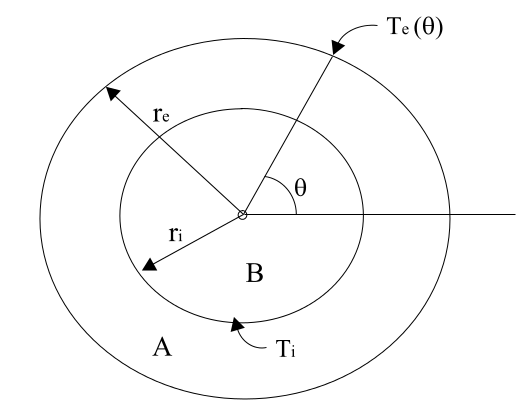
\includegraphics[width=0.6\columnwidth]{imagenes/horno.png}
\caption{Secci\'on circular del horno}
\end{center}
\end{figure}



El objetivo del trabajo práctico es implementar un programa que calcule la isoterma solicitada, conociendo las dimensiones del horno y las mediciones de temperatura en la pared exterior.

{\bf El Modelo}

Sea $r_e \in \mathbb{R}$ el radio exterior de la pared y sea $r_i \in \mathbb{R}$ el radio interior de la pared. Llamemos $T(r,\theta)$ a la temperatura en el punto dado por las coordenadas polares $(r,\theta)$, siendo $r$ el radio y $\theta$ el \'angulo polar de dicho punto. En el estado estacionario, esta temperatura satisface la ecuaci\'on del calor:

\begin{equation}\label{calor}
\frac{\partial^2T(r,\theta)}{\partial r^2}+\frac{1}{r}\frac{\partial T(r,\theta)}{\partial r}+\frac{1}{r^2}\frac{\partial^2T(r,\theta)}{\partial \theta^2} = 0 
\end{equation}


Si llamamos $T_i \in \mathbb{R}$ a la temperatura en el interior del horno (sector B) y $T_e : [0,2\pi] \rightarrow \mathbb{R}$ a la funci\'on de temperatura en el borde exterior del horno (de modo tal que el punto $(r_e,\theta)$ tiene temperatura $T_e(\theta)$), entonces tenemos que

\begin{equation}
T(r,\theta) = T_i \;\;\;\;\;para\;todo\;punto\;(r,\theta)\;con\;r\leq r_i
\end{equation}
\begin{equation}
T(r_e,\theta) = T_e(\theta) \;\;\;\;\;\;para\;todo\;punto\;(r_e,\theta)
\end{equation}


El problema en derivadas parciales dado por la primera ecuaci\'on con las condiciones de contorno presentadas recientemente, permite encontrar la funci\'on $T$ de temperatura en el interior del horno (sector A), en funci\'on de los datos mencionados en esta secci\'on.

Para resolver este problema computacionalmente, discretizamos el dominio del problema (el sector A) en coordenadas polares. Consideramos una partici\'on $0 = \theta_0 < \theta_1 < ... < \theta_n = 2\pi$ en $n$ \'angulos discretos con $\theta_k-\theta_{k-1} = \Delta\theta$ para $k = 1,...,n$, y una partici\'on $r_i = r_0 < r_1 < ... < r_m = r_e$ en $m+1$ radios discretos con $r_j - r_{j-1} = \Delta r$ para $j = 1,...,m$.

\medskip

El problema ahora consiste en determinar el valor de la funci\'on $T$ en los puntos de la discretizaci\'on $(r_j,\theta_k)$ que se encuentren dentro del sector A. Llamemos $t_{jk} = T(r_j,\theta_k)$ al valor (desconocido) de la funci\'on $T$ en el punto $(r_j,\theta_k)$.

\medskip

Para encontrar estos valores, transformamos la ecuaci\'on (\ref{calor}) en un conjunto de ecuaciones lineales sobre las inc\'ognitas $t_{jk}$, evaluando (\ref{calor}) en todos los puntos de la discretizaci\'on que se encuentren dentro del sector A. Al hacer esta evaluaci\'on, aproximamos las derivadas parciales de $T$ en (\ref{calor}) por medio de las siguientes f\'ormulas de diferencias finitas:


\begin{equation}
\frac{\partial^2T(r,\theta)}{\partial r^2}(r_j,\theta_k) \cong \frac{t_{j-1,k}-2t_{jk}+t_{j+1,k}}{(\Delta r)^2}
\end{equation}

\begin{equation}
\frac{\partial T(r,\theta)}{\partial r}(r_j,\theta_k) \cong \frac{t_{j,k}-t_{j-1,k}}{\Delta r}
\end{equation}

\begin{equation}
\frac{\partial^2T(r,\theta)}{\partial \theta^2}(r_j,\theta_k) \cong \frac{t_{j,k-1}-2t_{jk}+t_{j,k+1}}{(\Delta \theta)^2}
\end{equation}



Es importante notar que los valores de las inc\'ognitas son conocidos para los puntos que se encuentran sobre el borde exterior de la pared, y para los puntos que se encuentren dentro del sector B. Al realizar este procedimiento, obtenemos un sistema de ecuaciones lineales que modela el problema discretizado. La resoluci\'on de este sistema permite obtener una aproximaci\'on de los valores de la funci\'on $T$ en los puntos de la discretizaci\'on.

{\bf Enunciado}

Se debe implementar un programa en \verb+C+ o \verb-C++- que tome como entrada los par\'ametros del problema ($r_i$, $r_e$, $m+1$,
$n$, valor de la isoterma buscada, $T_i$, $T_e(\theta)$) que calcule la temperatura dentro de la pared del horno utilizando el
modelo propuesto en la secci\'on anterior y que encuentre la isoterma buscada en funci\'on del resultado obtenido del
sistema de ecuaciones. El m\'etodo para determinar la posici\'on de la isoterma queda a libre elecci\'on de cada grupo y
debe ser explicado en detalle en el informe.

El programa debe formular el sistema obtenido a partir de las ecuaciones (1) - (6) y considerar dos m\'etodos posibles
para su resoluci\'on: mediante el algoritmo cl\'asico de Eliminaci\'on Gaussiana y la Factorizaci\'on LU. Finalmente, el
programa escribir\'a en un archivo la soluci\'on obtenida con el formato especificado en la siguiente secci\'on.

Como ya se ha visto en la materia, no es posible aplicar los m\'etodos propuestos para la resoluci\'on a cualquier
sistema de ecuaciones. Sin embargo, la matriz del sistema considerado en el presente trabajo cumple con ser diagonal dominante (no
estricto) y que, ordenando las variables y ecuaciones convenientemente, es posible armar un sistema de ecuaciones cuya matriz
posee la propiedad de ser \emph{banda}. Luego, se pide demostrar (o al menos dar un esquema de la demostraci\'on)
el siguiente resultado e incluirlo en el informe:

\begin{proposition}
Sea $A \in \mathbb{R}^{n \times n}$ la matriz obtenida para el sistema definido por (1)-(6). Demostrar que es posible
aplicar Eliminaci\'on Gaussiana sin pivoteo.\footnote{Sugerencia: Notar que la matriz es diagonal dominante (no
estrictamente) y analizar qué sucede al aplicar un paso de Eliminaci\'on Gaussiana con los elementos de una fila.} 
\end{proposition}

La soluci\'on del sistema de ecuaciones permitir\'a saber la temperatura en los puntos de la discretizaci\'on. Sin embargo,
nuestro inter\'es es calcular la isoterma 500, para poder determinar si la estructura se encuentra en peligro. Luego, se pide lo siguiente:
\begin{itemize}
\item Dada la soluci\'on del sistema de ecuaciones, proponer una forma de estimar en cada \'angulo de la discretizaci\'on la posici\'on de la 
isoterma 500.
\item En funci\'on de la aproximaci\'on de la isoterma, proponer una forma (o medida) a utilizar para evaluar la peligrosidad de la estructura
en funci\'on de la distancia a la pared externa del horno.
\end{itemize}


En funci\'on de la experimentaci\'on, se busca realizar dos estudios complementarios: por un lado, analizar c\'omo se comporta el sistema y, por otro, 
cu\'ales son los requerimientos computacionales de los m\'etodos. Se pide como m\'inimo realizar los siguientes experimentos:
\begin{enumerate}
\item Comportamiento del sistema.
\begin{itemize}
\item Considerar al menos dos instancias de prueba, generando distintas discretizaciones para cada una de ellas y
comparando la ubicaci\'on de la isoterma buscada respecto de la pared externa del horno. Se sugiere presentar gr\'aficos
de temperatura o curvas de nivel para los mismos, ya sea utilizando las herramientas provistas por la c\'atedra o
implementando sus propias herramientas de graficaci\'on. 
\item Estudiar la proximidad de la isoterma buscada respecto de la pared exterior del horno en funci\'on de distintas 
granularidades de discretizaci\'on y las condiciones de borde. 
\end{itemize}
\item Evaluaci\'on de los m\'etodos.
\begin{itemize}
\item Analizar el tiempo de c\'omputo requerido para obtener la soluci\'on del sistema en funci\'on de la granularidad de 
la discretizaci\'on. Se sugiere presentar los resultados mediante gr\'aficos de tiempo de c\'omputo en funci\'on de alguna 
de las variables del problema.
\item Considerar un escenario similar al propuesto en el experimento 1. pero donde las condiciones de borde (i.e., $T_i$ y $T_e(\theta)$)
cambian en distintos instantes de tiempo. En este caso, buscamos obtener la secuencia de estados de la temperatura en
la pared del horno, y la respectiva ubicaci\'on de la isoterma especificada. Para ello, se considera una secuencia de $ninst$
vectores con las condiciones de borde, y las temperaturas en cada estado es la soluci\'on del correspondiente sistema de
ecuaciones. Se pide formular al menos un experimento de este tipo, aplicar los m\'etodos de resoluci\'on propuestos de
forma conveniente y compararlos en t\'erminos de tiempo total de c\'omputo requerido para distintos valores de $ninst$.
\end{itemize}
\end{enumerate}

De manera opcional, aquellos grupos que quieran ir un poco m\'as all\'a pueden considerar trabajar y desarrollar alguno(s) 
de los siguientes puntos extra:
\begin{enumerate}
\item Notar que el sistema resultante tiene estructura \emph{banda}. Proponer una estructura para aprovechar este hecho en t\'erminos de la
\emph{complejidad espacial} y como se adaptar\'ian los algoritmos de Eliminaci\'on Gaussiana y Factorizaci\'on LU para reducir la
cantidad de operaciones a realizar.
\item Implementar dicha estructura y las adaptaciones necesarias para el algoritmo de Eliminaci\'on Gaussiana.
\item Implementar dicha estructura y las adaptaciones necesarias para el algoritmo de Factorizaci\'on LU. 
\end{enumerate}

Finalmente, se deber\'a presentar un informe que incluya una descripci\'on detallada de los m\'etodos implementados y
las decisiones tomadas, el m\'etodo propuesto para el c\'alculo de la isoterma buscada y los experimentos realizados,
junto con el correspondiente an\'alisis y siguiendo las pautas definidas en el archivo \verb+pautas.pdf+.

{\bf Programa y formato de archivos}

Se deber\'an entregar los archivos fuentes que contengan la resoluci\'on del trabajo pr\'actico. El ejecutable tomar\'a
tres par\'ametros por l\'inea de comando, que ser\'an el archivo de entrada, el archivo de salida, y el m\'etodo a
ejectutar (0 EG, 1 LU).

El archivo de entrada tendr\'a la siguiente estructura:
\begin{itemize}
\item La primera l\'inea contendr\'a los valores $r_i$, $r_e$, $m+1$, $n$, $iso$, $ninst$, donde $iso$ representa el
valor de la isoterma buscada y $ninst$ es la cantidad de instancias del problema a resolver para los par\'ametros dados.
\item A continuaci\'on, el archivo contendr\'a $ninst$ l\'ineas, cada una de ellas con $2n$ valores, los primeros $n$ indicando los
valores de la temperatura en la pared interna, i.e., $T_i(\theta_0),T_i(\theta_1),\dots,T_i(\theta_{n-1})$, seguidos de $n$ valores
de la temperatura en la pared externa, i.e., $T_e(\theta_0)$,$T_e(\theta_1)$,$\dots$,$T_e(\theta_{n-1})$.
\end{itemize}

El archivo de salida obligatorio tendr\'a el vector soluci\'on del sistema reportando una componente del mismo por
l\'inea. En caso de $ninst > 1$, los vectores ser\'an reportados uno debajo del otro.

Junto con el presente enunciado, se adjunta una serie de scripts hechos en \verb+python+ y un conjunto instancias de
test que deber\'an ser utilizados para la compilaci\'on y un testeo b\'asico de la implementaci\'on. Se recomienda leer
el archivo \verb+README.txt+ con el detalle sobre su utilizaci\'on.

{\bf \underline{Fechas de entrega}}
\begin{itemize}
\item \emph{Formato Electr\'onico:} Jueves 3 de Septiembre de 2015, hasta las 23:59 hs, enviando el trabajo (informe +
c\'odigo) a la direcci\'on \verb+metnum.lab@gmail.com+. El subject del email debe comenzar con el texto \verb+[TP1]+
seguido de la lista de apellidos de los integrantes del grupo.
\item \emph{Formato f\'isico:} Viernes 4 de Septiembre de 2015, de 17:30 a 18:00 hs.
\end{itemize}

\noindent \textbf{Importante:} El horario es estricto. Los correos recibidos despu\'es de la hora indicada ser\'an
considerados re-entrega. Los grupos deben ser de 3 o 4 personas, sin excepci\'on. Es indispensable que los trabajos
pasen satisfactoriamente los casos de test provistos por la c\'atedra.


\newpage
\section{Código C++} \label{sec:codigo}
\subsection{alto_horno.h}
\lstinputlisting[language=C++]{codigo/alto-horno.h}
\subsection{alto_horno.cpp}
\lstinputlisting[language=C++]{codigo/alto-horno.cpp}
\subsection{sistema_ecuaciones.h}
\lstinputlisting[language=C++]{codigo/sistema-ecuaciones.h}
\subsection{sistema_ecuaciones.cpp}
\lstinputlisting[language=C++]{codigo/sistema-ecuaciones.cpp}


\end{document}
